% !TEX root = main.tex

% COMPLETE

\newcommand{\mdaarchitectures}{$128$D embeddings were generated by $256$-$128$, $512$-$128$, $1024$-$128$, $256$-$256$-$128$, $512$-$256$-$128$ and $512$-$512$-$128$ MDAE architectures. $256$D embeddings were generated by $256$-$256$, $512$-$256$ and $512$-$512$-$256$ MDAE architectures.}

\chapter{Feature learning from graphs using unsupervised neural networks}
\chaptermark{Feature learning from graphs}
\label{chapter:network-fusion}

% \section*{Abbreviations}\label{abbreviations}
% \addcontentsline{toc}{section}{Abbreviations}

% \begin{table}[ht!]
%     \centering
%     \begin{tabular}{ll}
%         \toprule
%         \textbf{Abbreviation} & \textbf{Phrase} \\ \midrule
%         % AE & autoencoder \\
%         deepNF & deep network fusion \\
%         % FN & false negatives \\
%         % FP & false positives \\
%         % FYPO & fission yeast phenotype ontology \\
%         GO & Gene Ontology \\
%         mAUPR & micro-averaged area under the precision-recall curve \\
%         MAUPR & macro-averaged area under the precision-recall curve \\
%         MDAE & multimodal deep autoencoder \\
%         MIPS & Mammalian Protein-Protein Interaction Database \\
%         MLP & multi-layer perceptron \\
%         % PCNet & parsimonious composite network \\
%         % PPMI & positive pointwise mutual information \\
%         % RBF & radial basis function \\
%         % ReLU & rectified linear unit \\
%         % RWR & random walks with restart \\
%         % SGD & stochastic gradient descent \\
%         \emph{S. cerevisiae} & \emph{Saccharomyces cerevisiae} \\
%         \emph{S. pombe} & \emph{Schizosaccharomyces pombe} \\
%         STRING & Search Tool for the Retrieval of Interacting Genes/Proteins \\
%         SVM & support vector machine \\
%         % TN & true negatives \\
%         % TP & true positives \\
%         \bottomrule
%     \end{tabular}
%     % \addtocounter{table}{-1}
% \end{table}

\section{Introduction}

In this chapter, we explore a state-of-the-art protein function prediction method, deep network fusion (deepNF), that uses protein networks as its sole training data.

Graphs are ubiquitous data structures that are suited to modelling problems that are high-dimensional and sparse.
As such, graphs are an ideal data structure to represent the myriad protein interactions that give rise to biological life.
However, due to many biological and experimental factors, networks are models that try to capture as many of the true interactions that proteins make, but are often incomplete.

Given some protein network, one may want to perform link prediction to predict additional interactions that proteins might make, but are missing from the network.
In the past decade, machine learning has become the de facto framework to model prediction problems.
Due to memory constraints, it may not be practically feasible to represent graphs as dense matrices of features, as is required for many types of machine learning algorithms.
For example, storing a dense adjacency matrix of a $10^6$ node graph in $64$-bit precision requires $80$ GB of memory.
Furthermore, even if dense graph matrices can be stored, machine learning algorithms may not be able to learn from them because of high sparsity, the curse of dimensionality and the `many features; few examples' problem.

Classically, hand engineered features would be calculated from graphs for use in machine learning.
For example, in link prediction, one may want to encode the strength of interactions between pairs of nodes.
Alternatively, in node classification, one may want to encode information about the local and global context of nodes.
Encoding this information may be inflexible, biased, time-consuming or not suited to vector representations.
Below, we introduce a variety of modern approaches to applying machine learning to graphs.

\subsection{Guilt by association}

Guilt by association relies on a notion of similarity between entities.
Metadata annotated to one entity can be transferred to the other entities that are sufficiently similar, because these entities are guilty by association.
This approach is employed by GO \cite{Ashburner2000}, where 40\% of all annotations are assigned to homologous proteins \cite{Peled2016}.

Graphs can be used to predict labels using guilt by association \cite{Lehtinen2015,Heriche2014,Mostafavi2008,Gligorijevic2018,Cho2016}, where edge weights and the network topology encode similarities between nodes.
Under this framework, nodes that are either directly connected, close by in the network or appear in similar network contexts are guilty by association.
Functional annotations attached to one node can be transferred to the other associated nodes.
However, opponents of guilt by association approaches have shown that functional information is not encoded throughout the network, but rather is concentrated to a small number of specific edges \cite{Gillis2012}.

\subsection{Graph embeddings}

Embedding methods learn representations of nodes that encode structural information about the graph \cite{Hamilton2017}.
Embeddings are vectors that represent a set of latent features that are automatically learnt from the graph.
The goal is to optimise the embedding, such that relationships in the embedding space recapitualate relationships in the graph space.
Protein network graph embeddings of have been used previously for function prediction \cite{Cho2016,Gligorijevic2018}.
The crucial advance of graph embedding methods is that the function that maps nodes to the embedding space is learnt from the data in an unsupervised way.
Graph embedding methods are not domain-specific, so they can be applied to any graph.
Low-dimensional embeddings tend to be learnt, where on the order of $10^2-10^3$ latent dimensions are used.
These embeddings are small enough such that they can be used to train off the shelf machine learning models.
Alternatively embeddings can be used to calculate distances between nodes---in terms of the differences in their network contexts---with applications in clustering.

\subsection{Encoder-decoders}
% https://www-cs.stanford.edu/people/jure/pubs/graphrepresentation-ieee17.pdf

Encoder-decoders are a general framework used by embedding methods \cite{Hamilton2017}.
In encoder-decoders, the encoder first maps nodes to low-dimensional embeddings, followed by reconstruction of the original data by the decoder, using only the embeddings.
Transitively, if the original data can be reconstructed by the encoder-decoder model, then the embeddings must contain all salient information in the graph.
As such, the embeddings can be used for machine learning.

The encoder and decoder functions are learnt in an unsupervised way from the data using an optimisation process.
In order to do this, a loss function must be defined to measure the difference between the original data and its reconstruction from the embeddings.
The encoder and decoder functions are then optimised to minimise the reconstruction loss, and,
concomitantly, the embeddings are improved.

Autoencoders are a type of encoder-decoder model implemented using an unsupervised neural network model.
In this chapter, we make extensive use of deepNF, an autoencoder-based method that learns node embeddings across multiple graphs.
We introduced deepNF in \ref{sec:intro-deepnf} and showed an overview of the autoencoder architecture in \ref{fig:deepNF}.

\subsection{Contributions}

Functional association data are powerful predictors of protein function.
Here, we perform feature learning from protein networks using multimodal deep autoencoders (MDAEs) to embed proteins into a latent space, according to their context across multiple networks.
Using these embeddings, we train supervised machine learning models to predict protein function in budding and fission yeast.
We began by replicating the published performance of deepNF \cite{Gligorijevic2018} at predicting \emph{S. cerevisiae} protein function.
Following this, we improved upon deepNF in three ways.
Firstly, we showed that smaller MDAE architectures, and secondly, smaller embedding dimensions, achieve comparable performance to deepNF.
Thirdly, we found that protein functions can be predicted using structured learning with the same performance as predicting each function using a separate classifier.
This not only reduced training and prediction time, but also allowed non-linear correlations to be learnt between features and labels.
We then applied this improved model to predict \emph{S. pombe} protein function using structured learning.
Finally, we attempted to improve the predicted protein functions by learning features from a larger set of orthogonal types of protein interactions.
We take this approach forward to \ref{chapter:yeast}, where we predict \emph{S. pombe} protein function in combination with phenotypic and protein evolution data.


\section{Methods}

\subsection{Protein functional association data}
\label{network-data}

Protein networks were prepared as in deepNF \cite{Gligorijevic2018}.
Interactions from the Search Tool for the Retrieval of Interacting Genes/Proteins (STRING) database \cite{Szklarczyk2017} were used.
STRING has seven interaction types:

\begin{itemize}
    \item `neighborhood',
    \item `fusion',
    \item `cooccurence',
    \item `coexpression',
    \item `experimental',
    \item `database', and
    \item `textmining' (not used in this study).
\end{itemize}

Briefly, adjacency matrices were generated by the following protocol for each of the six interaction types:

\begin{enumerate}
\item Protein IDs were sorted alphabetically and converted to numerical node IDs.
\item Edge weights were normalised to the interval $[0,1]$.
\item Each adjacency matrix was scaled so that rows sum to unity.
\item Random walks with restart
\[
P^{(t)} = \alpha P^{(t+1)}A + (1-\alpha)I,
\]
was applied to each adjacency matrix $A$.
$P^{(t)}$ is a matrix whose rows are the probabilities for a random walk from the $i$th protein reaching the $j$th protein after $t$ steps.
$\alpha=0.98$ is the restart probability.
Random walks with restart was run for $t=3$ time steps.
\item Positive pointwise mutual information was applied to $P$ to remove low probability edges.
\end{enumerate}

STRING v9.1 \cite{Franceschini2013} was used to generate \emph{Saccharomyces cerevisiae} (\emph{S. cerevisiae}) adjacency matrices.
Despite STRING v10.5 \cite{Szklarczyk2015} being available when this work was performed, deepNF used STRING v9.1 in \cite{Gligorijevic2018}, so we also used v9.1 so that we could compare the performance of our models to deepNF.
STRING v10.5 \cite{Szklarczyk2015} was used to generate \emph{Schizosaccharomyces pombe} (\emph{S. pombe}) matrices.
A number of additional \emph{S. pombe} networks were also prepared using the same protocol:

\begin{itemize}
    \item Genetic interactions from BioGRID \cite{Oughtred2018}.
    \item Gene expression correlations from an \emph{S. pombe} gene expression meta-analysis \cite{Pancaldi2010}.
    \item Fission yeast phenotype ontology annotations of experimentally observed phenotypes \cite{Harris2013}. Note that these annotations are disjoint from GO annotations \cite{Carbon2018}.
\end{itemize}


\subsection{Protein function data}

For \emph{S. cerevisiae}, Mammalian Protein-Protein Interaction Database (MIPS) terms \cite{Pagel2005; Ruepp2004} were divided into three levels according to the number of proteins they are annotated to (\ref{table:MIPS}).
The last MIPS publication is from 2005 \cite{Pagel2005}, so is very outdated.
deepNF was benchmarked in \cite{Gligorijevic2018} using MIPS annotations so that its performance could be compared to another method, Mashup \cite{Cho2016}, that also predicted MIPS annotations.
As such, we chose to predict MIPS annotations for \emph{S. cerevisiae}.

\begin{table}[ht!]
    \centering
    \caption{%
        \emph{S. cerevisiae} MIPS term annotations.
    }
    \label{table:MIPS}
    \begin{tabular}{ccc}
        \toprule
        \textbf{Level} & \textbf{Number of proteins term is annotated to} & \textbf{Number of terms} \\
        \midrule
        $1$ & $101-300$ & $17$ \\
        $2$ & $31-100$ & $74$ \\
        $3$ & $11-30$ & $154$ \\
        \bottomrule
    \end{tabular}
\end{table}

As neither deepNF or Mashup benchmarked \emph{S. pombe}, rather than use MIPS annotations, we chose to use Gene Ontology (GO) annotations because the data is more comprehensive and up-to-date.
GO terms were divided into three levels per ontology (\ref{table:GO}) using the same criteria as \emph{S. cerevisiae} MIPS annotations.
Annotations with experimental (EXP, IDA, IPI, IMP, IGI, IEP, HDA and HMP) and curated (IC and TAS) evidence codes were used.

\begin{table}[hbt!]
    \centering
    \caption{%
        \emph{S. pombe} GO term annotations for each of the biological process (P), molecular function (F) and cellular component (C) ontologies.
    }
    \label{table:GO}
    \begin{tabular}{cccc}
        \toprule
        \textbf{Level} & \textbf{Number of proteins term is annotated to} & \textbf{Ontology} & \textbf{Number of terms} \\
        \midrule
        $1$ & $101-300$ & P & $7$ \\
        & & F & $6$ \\
        & & C & $7$ \\
        \midrule
        $2$ & $31-100$ & P & $34$ \\
        & & F & $27$ \\
        & & C & $25$ \\
        \midrule
        $3$ & $11-30$ & P & $97$ \\
        & & F & $61$ \\
        & & C & $48$ \\
        \bottomrule
    \end{tabular}
\end{table}

\subsection{Feature learning from graphs using unsupervised neural networks}

We used autoencoders for unsupervised feature learning from graphs, each representing a different type of protein interaction.
One method that implements this type of model is deepNF \cite{Gligorijevic2018}, which we introduced in \ref{sec:intro-deepnf}.
Here, we replicate deepNF's published results, improve some of its properties, and then apply it to predict \emph{S. pombe} protein function.
Briefly, deepNF uses an MDAE to learn a small number of informative features ($10^2$) from a large number of protein interactions ($10^4 - 10^5$).
An overview of deepNF is shown in \ref{fig:deepNF}.

\subsubsection{Autoencoder architecture notation}\label{notation}

For brevity, MDAE architectures are referred to using the hidden layers in the encoding portion of the autoencoder and the number of neurons in each hidden layer.
For example, the MDAE architecture used in deepNF is a `$2000$-$600$ MDAE' that embeds each protein in a $600$D space using two hidden layers of $2000$ neurons and $600$ neurons.
Let $n$ be the number of proteins in some organism and $g$ be the number of input network adjacency matrices. The overall architecture of the $2000$-$600$ MDAE is
\[
\text{Input: }g{[}n{]} \rightarrow g{[}2000{]} \rightarrow \text{Encoding: }600 \rightarrow g{[}2000{]} \rightarrow \text{Output: }g{[}n{]},
\]
where the decoding portion is always the mirror image of the encoding portion.

In words, the $2000$-$600$ MDAE takes $g$ adjacency matrices with shape $[n \times n]$ as input,
processes each matrix with a separate 2000 neuron layer and passes the outputs of these $g$ layers to a single $600$ neuron encoding layer.
For each of the $n$ proteins, this layer outputs a $600$D vector, which is the of each protein in a $600$D space.
Embeddings are then passed to $g$ $2000$ neuron layers, whose outputs are used to reconstruct the $g$ adjacency matrices.
deepNF uses $g=6$ adjacency matrices from six types of interaction from STRING (\ref{network-data}).

\subsubsection{Autoencoders}
\label{autoencoder}

% An MDAE was was used to fuse multiple adjacency matrices that capture different notions of protein interactions. The MDAE was then used to generate embeddings for all proteins.
% Neural networks and autoencoder architectures are introduced extensively elsewhere. The MDAE architecture and training routine were often varied---please refer to the results of a particular experiment for details. When using PCNet \cite{Huang2018} as input, a vanilla (taking a single adjacency matrix as input) autoencoder was used instead of an MDAE.

Autoencoders are a type of neural network that consists of an encoder and a decoder.
The network tries to reconstruct the input as best it can.
Reconstructions are rarely perfect, but that is not why autoencoders are used.
Instead, they are used to learn a set of latent features from the input data.
To do this, constraints are imposed on the encoder part of the network that prevent a simple identity function from being learnt.
In this work, we impose a size contraint on the encoder, where inputs are embedded into a low-dimensional latent space.
As such, the reconstuctions will be lossy, but the embedding will be forced to be informative.

Sigmoid activations were always used on the output layer.
Autoencoders were trained using data from $90\%$ of proteins.
The remaining $10\%$ of proteins were used as a validation set to monitor training.
Models were trained using binary crossentropy loss.
Batch sizes of $128$ examples were used.
Unless specified otherwise:

\begin{itemize}
    \item Rectified linear unit activation functions were used on hidden layers.
    \item The Adam optimiser \cite{Kingma2014} was used.
    \item Models were trained for $500$ epochs, where the weights from the epoch with the lowest validation loss were used to generate the embeddings.
\end{itemize}

\noindent Models were implemented in Python v3.6 \cite{Python} using Keras v2.1.5 \cite{chollet2015keras}
(TensorFlow v1.8.0 \cite{GoogleResearch2015} backend).

\subsection{Protein function prediction}

Protein functions were predicted using supervised machine learning.
Models were trained to learn a mapping from protein embeddings, generated by MDAs, to protein functions.

\subsubsection{Performance metrics}
\label{performance}

Classifier performance was measured using four metrics:

\begin{itemize}
    \item Macro-averaged area under the precision-recall curve (MAUPR), calculated as the mean AUPR for each class separately.
    \item Micro-averaged area under the precision-recall curve (mAUPR), by aggregating all classes together and calculating a single AUPR.
    \item Accuracy, defined as $\frac{\text{TP} + \text{TN}}{|\text{P}| + |\text{N}|}$, where TP are true positives of the positive class P, and TN are true negatives of the negative class N. More specifically, the subset accuracy is calculated, where a multiclass prediction is counted as correct if and only if the predictions match the known labels across all classes.
    \item f1 score, defined as $\frac{2 \times \text{precision} \times \text{recall}}{\text{precision} + \text{recall}}$, where precision is $\frac{\text{TP}}{\text{TP} + \text{FP}}$ and recall is $\frac{\text{TP}}{\text{TP} + \text{FN}}$.
\end{itemize}

\subsubsection{Support vector machines}
\label{support-vector-machine}

Support vector machines (SVMs; \ref{sec:intro-svm}) were trained using the one-vs-rest multiclass strategy.
The radial basis function kernel was used and hyperparameters were estimated using an exhaustive grid search of $C = \{1, 5, 10, 50, 100\}$ and $\gamma = \{0.001, 0.005, 0.01, 0.05, 0.1\}$, selecting values that maximised mAUPR.
The soft-margin penalty $C$ is common to all SVMs and controls the penalty applied to errors, with large values producing decision boundaries with a small margin between the two classes.
The radial basis function kernel parameter $\gamma$ controls the influence of the data points, with high values increasing the locality of influence that the support vectors have on kernel values.
Models were evaluated using $10$ independent trials of $5$-fold cross-validation with $80\%$ of the data as a training set and $20\%$ of the data as a test set.
Models were implemented in Python 3.6 \cite{Python} using scikit-learn 0.19.1.

\subsubsection{Multi-layer perceptrons}
\label{multi-layer-perceptron}

Multi-layer perceptrons (MLPs) were trained using structured learning.
An MLP architecture was used that had two hidden layers of $512$ and $256$ neurons.
Dropout was applied to the output of the first hidden layer with $P(\text{dropout}) = 0.5$.
Models were trained using binary crossentropy loss and Adam optimiser.
Batch sizes of $128$ were used.
The dropout rate and batch size were chosen empirically.
Models were evaluated using $10$ independent trials of 5-fold cross-validation with $80\%$ of the data as a training set (of which $20\%$ was used as a validation set) and $20\%$ of the data as a test set.
Loss was calculated after each epoch using the training and validation data.
Overfitting was controlled by early stopping when the validation loss no longer decreased, using a patience of $20$ epochs.
Weights from the epoch with lowest validation loss were used.
Models were implemented in Python v3.6 \cite{Python} using Keras v2.1.5 \cite{chollet2015keras}
(TensorFlow v1.8.0 \cite{GoogleResearch2015} backend).

% \subsection{PCNet}\label{pcnet}
%
% PCNet \cite{Huang2018} is a recent and novel network fusion strategy that generate a `parsimonious composite' network, or PCNet, from multiple networks. The PCNet is generated by taking the intersection over the sets of edges from the STRING network and each additional network. The predictive performance of the PCNet is higher than the STRING network alone. This is in contrast to a composite network formed by taking the union over the sets of edges---which leads to no improvement in predictive performance.


\section{Results}

Each experiment performed in this chapter had a common structure:

\begin{enumerate}
    \item Use an MDAE for unsupervised protein feature learning from multiple protein networks.
    \item Generate a small number of informative features for each protein.
    \item Train a classifier to predict protein function using these features.
\end{enumerate}

\subsection{Published performance of deepNF was replicated}
\label{replicate-deepnf-results}

We replicated the results of deepNF at predicting MIPS function annotations using the published model and parameters.
A $2000$-$600$ MDAE with sigmoid activations was trained using stochastic gradient descent for $10$ epochs.
The reconstruction loss for the MDAE on the training data and a validation set shows that the MDAE is not fully trained because the loss has not levelled out by the \nth{10} epoch (\ref{fig:replicate-deepNF-loss}).
Training for more epochs, until the validation loss is minimised, may improve the performance.

% \begin{table}[!hbt]
%     \centering
%     \caption{%MDAE parameters to replicate deepNF.}
%     \label{table:replicate-deepNF-params}
%     \begin{tabular}{ll}
%         \toprule
%         \textbf{Parameter} & \textbf{Value} \\
%         \midrule
%         MDAE architecture & 2000-600 \\
%         Activation function & Sigmoid \\
%         Optimiser & SGD \\
%         Epochs & 10 \\
%         \bottomrule
%     \end{tabular}
% \end{table}

\begin{figure}[!hbt]
    \centering
    \includegraphics[width=.6\textwidth]{./Chapter_network_fusion/cerevisiae/deepNF/180807_77cd62b/cerevisiae_MDA_arch_2000-600}
    \caption{%
        MDAE reconstruction loss when replicating deepNF results.
        Binary crossentropy loss on the validation set (solid line) and on the training set (dotted line).
        % A 2000-600 MDAE was trained on \emph{S. cerevisiae} data derived from six STRING networks and used to generate protein embeddings.
        % The reconstruction loss was calculated on a validation set consisting of 10\% of the available data.
    }
    \label{fig:replicate-deepNF-loss}
\end{figure}

The MDAE is not overfitting to the training data, so should be generalisable. When overfitting occurs, the validation loss increases, whilst the training loss continues to decrease.

When training for more epochs, overfitting should be controlled by early stopping or by saving the weights from the epoch with the lowest validation loss. Both strategies have their merits: training with early stopping is faster, but it is not possible to know whether the validation loss may begin to decrease again at a later epoch. Saving the weights from the best epoch may overcome the problem of not knowing how long to wait before early stopping, however, the model may need to be trained for a long time to be confident.

Proteins were embedded into a $600$D space by the MDAE, using weights from the \nth{10} epoch. Embeddings were used as features to train SVMs to predict MIPS terms. The one-vs-rest multiclass strategy was used, where classes are treated separately and one classifier is trained per class.
We successfully replicated results of deepNF published in \cite{Gligorijevic2018} for mAUPR, MAUPR, accuracy and f1 score.

% 10 independent trials of 5-fold cross-validation were performed (\ref{fig:replicate-deepNF-cv}). We successfully replicated the results of deepNF for mAUPR, MAUPR, accuracy and f1 score (shown as horizontal blue lines).

\begin{figure}[!ht]
    \centering
    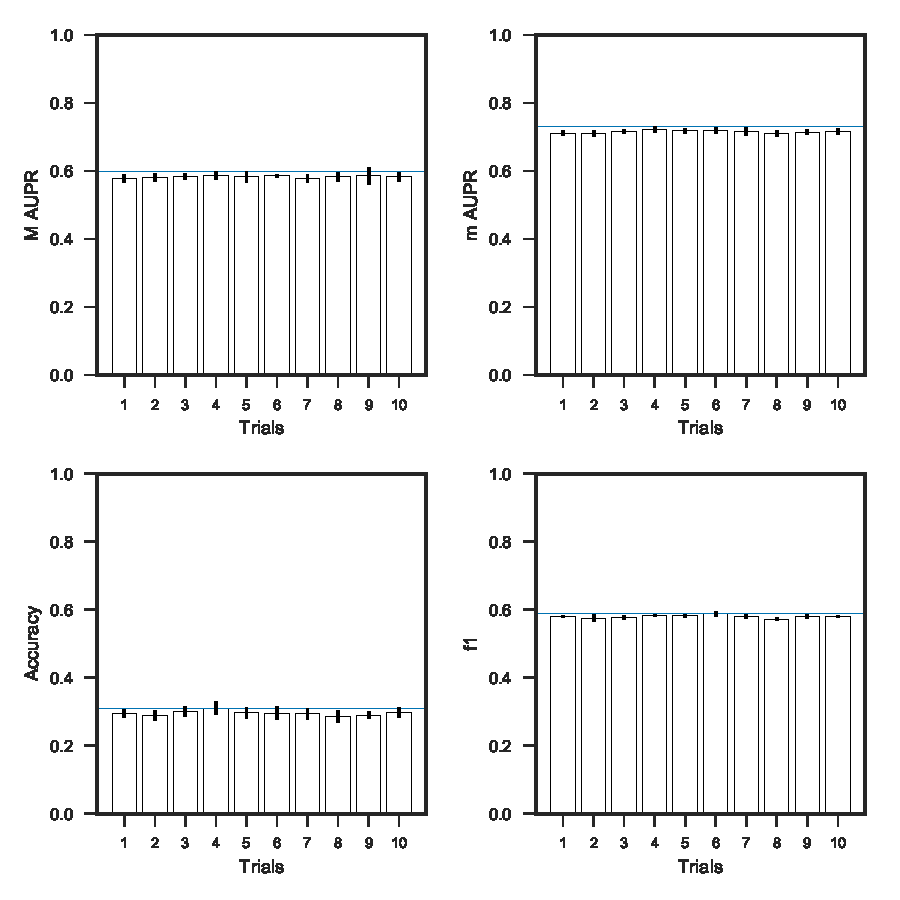
\includegraphics[width=\textwidth]{./Chapter_network_fusion/cerevisiae/classification/cv_cerevisiae_level1_MDA-2000-600-all-sigmoid-sgd}
    \caption{%
        Protein function prediction performance when replicating deepNF results for \emph{S. cerevisiae}.
        % Protein embeddings were used as features to train a one-vs-rest SVM to predict MIPS annotations.
        MIPS terms were divided into three levels according to the number of proteins that are annotated with each term.
        % : 101-300 proteins in level 1, 31-100 proteins in level 2, and 11-30 proteins in level 3.
        % 10 independent trials of 5-fold cross-validation were performed.
        Bars are the mean performance across $10$ independent trials of $5$-fold cross-validation and error bars are the standard deviation.
    }
    \label{fig:replicate-deepNF-cv}
\end{figure}

% \subsubsection{Improving the performance of deepNF with current best practices}\label{improving-the-performance-of-deepnf-with-current-best-practices}

% I replaced two outdated techniques that deepNF used in the MDAE with current best practices for neural networks in an attempt to improve prediction performance (\ref{table:best-practices-overview}).
%
% \begin{table}[!ht]
%     \centering
%     \caption{%Best practices: improving deepNF with current best practices.}
%     \label{table:best-practices-overview}
%     \begin{tabularx}{\textwidth}{lllX}
%         \toprule
%         & \textbf{deepNF} & \textbf{Replacement} & \textbf{Explanation} \\
%         \midrule
%         \textbf{Activation function} & Sigmoid & ReLU & Overcomes the problems of vanishing gradients associated with sigmoid activations, that squash the entire number line into the interval $[0,1]$ \\
%         \textbf{Optimiser} & SGD & Adam & More recent optimisers find the optimal direction and magnitude with which to update weights, allowing neural networks to train and converge faster \\
%         \bottomrule
%     \end{tabularx}
% \end{table}
%
% \begin{table}[!ht]
%     \centering
%     \caption{%Best practices: MDAE parameters.}
%     \label{table:best-practices}
%     \begin{tabular}{ll}
%         \toprule
%         \textbf{Parameter} & \textbf{Value} \\
%         \midrule
%         MDAE architecture & 2000-600 \\
%         Activation function & ReLU \\
%         Optimiser & Adam \\
%         Epochs & 20 \\
%         \bottomrule
%     \end{tabular}
% \end{table}
%
% The MDAE loss is improved when using ReLU and Adam (\ref{fig:best-practices-loss}), compared with sigmoid and SGD (\ref{fig:replicate-deepNF-loss}). The loss after one epoch is significantly better than the loss after 10 epochs with sigmoid and SGD, and continues to decrease gradually for the remaining epochs.
%
% \begin{figure}[!ht]
%     \centering
%     \includegraphics[width=.6\textwidth]{./Chapter_network_fusion/cerevisiae/deepNF/180808_fc6fe63/cerevisiae_MDA_arch_2000-600}
%     \caption{%Best practices: MDAE reconstruction loss. ReLU activation functions and the Adam optimiser was used. \losscerevisiae{2000-600}}
%     \label{fig:best-practices-loss}
% \end{figure}
%
% However, despite the MDAE loss being lower, the prediction performance was worse using these embeddings than using embeddings generated by an MDAE using sigmoid and SGD (\ref{fig:best-practices-cv}). The difference in performance may be due to the sparsity of embeddings generated by a ReLU encoding layer, because ReLU clips all negative outputs to zero.
%
% \begin{figure}[!ht]
%     \centering
%     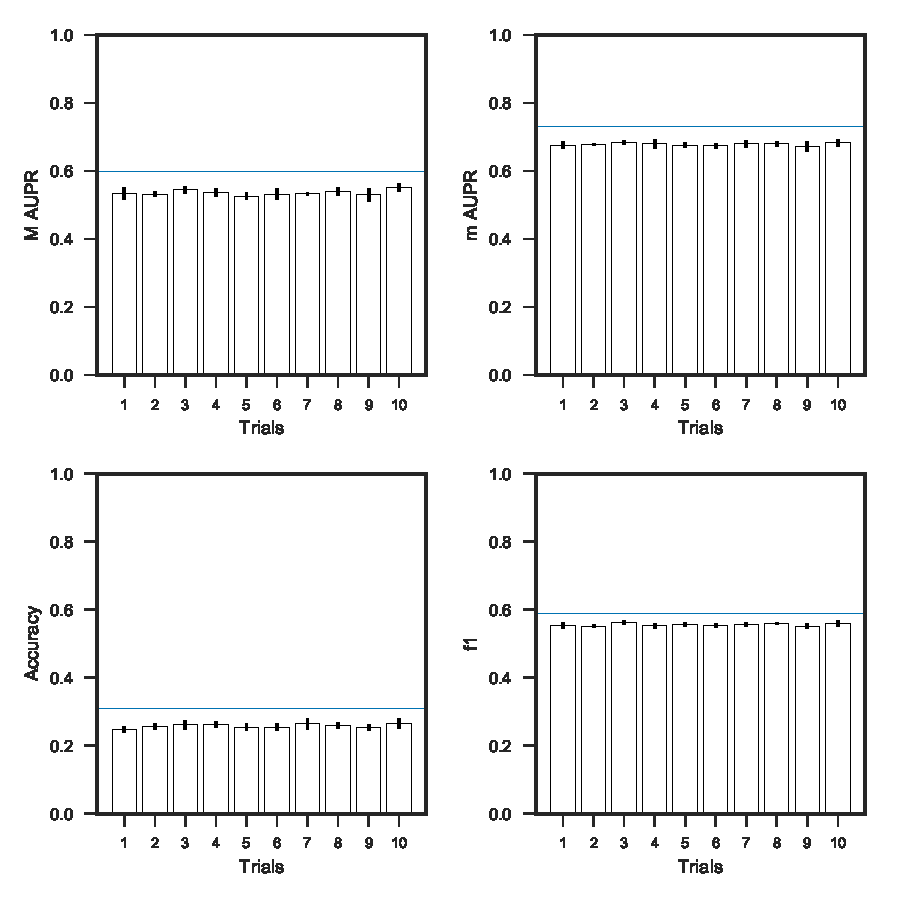
\includegraphics{./Chapter_network_fusion/cerevisiae/classification/cv_cerevisiae_level1_MDA-2000-600-best-practice}
%     \caption{%Best practices: cross-validation results. \cvmipssvm\ \cvlevelone\ \cvdeepnfcomparison}
%     \label{fig:best-practices-cv}
% \end{figure}
%
% \paragraph{Compare the effects of using sigmoid activations versus ReLU activations}\label{compare-the-effects-of-using-sigmoid-activations-versus-relu-activations}
%
% To investigate whether ReLU reduces performance, I compared the effects of using a sigmoid activation function on the output of the 600 neuron encoding layer with ReLU on the other layers (encoding-sigmoid) to using sigmoid activations on all layers (all-sigmoid) (\ref{table:relu-vs-sigmoid}). Both MDAs achieved a similar loss (\ref{fig:relu-vs-sigmoid-loss}). Interestingly, the encoding-sigmoid MDAE took longer to converge than the all-sigmoid MDAE. Previously, I have observed that ReLU neural networks have a lag of a small number of epochs before rapidly converging, which may be attributed to ReLU clipping negative outputs produced by randomly initialised layer weights.
%
% \begin{table}[!ht]
%     \centering
%     \caption{%MDAE parameters for comparing the effects of using sigmoid activations versus ReLU activations.}
%     \label{table:relu-vs-sigmoid}
%     \begin{tabular}{ll}
%         \toprule
%         \textbf{Parameter} & \textbf{Value} \\
%         \midrule
%         MDAE architecture & 2000-600 \\
%         Activation function & Encoding-sigmoid: sigmoid and ReLU, All-sigmoid: sigmoid \\
%         Optimiser & Adam \\
%         Epochs & 20 \\
%         \bottomrule
%     \end{tabular}
% \end{table}
%
% \begin{figure}[!ht]
%     \centering
%     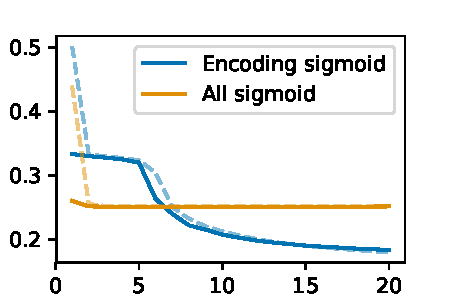
\includegraphics[width=.6\textwidth]{./Chapter_network_fusion/cerevisiae/deepNF/180808_eec3d7b/cerevisiae_MDA_arch_2000-600_activation-functions}
%     \caption{%Activation functions: MDAE reconstruction loss. \emph{Blue:} loss for MDAE using sigmoid activations on the output of the encoding layer and ReLU activations on other layers. \emph{Orange:} loss for MDAE using sigmoid activations on the output of all layers. \losscerevisiae{2000-600}}
%     \label{fig:relu-vs-sigmoid-loss}
% \end{figure}
%
% The prediction performance using embeddings generated by both MDAs is lower than deepNF (\ref{fig:relu-vs-sigmoid-cv}). This suggests that using Adam instead of SGD has a large impact on the protein embeddings produced by the MDAE. Again, we see that despite the MDAE having a lower loss when using Adam, the resulting protein embeddings are not as informative.
%
% \begin{figure}[!ht]
%     \centering
%     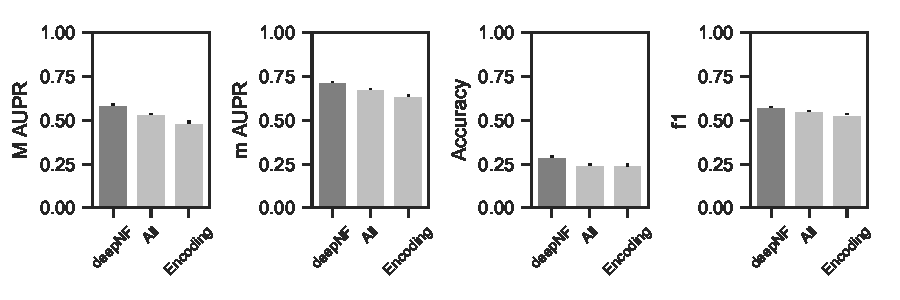
\includegraphics{./Chapter_network_fusion/cerevisiae/classification/cv_cerevisiae_level1_MDA-2000-600-activation-functions}
%     \caption{%Activation functions: cross-validation results. \cvmipssvm\ \cvlevelone\ \cvdeepnfcomparison}
%     \label{fig:relu-vs-sigmoid-cv}
% \end{figure}
%
% \paragraph{Compare the effects of using SGD optimiser versus Adam optimiser}\label{compare-the-effects-of-using-sgd-optimiser-versus-adam-optimiser}
%
% To confirm whether the choice of optimiser affects the quality of the protein embeddings, I compared MDAs trained using SGD or Adam (\ref{table:sgd-vs-adam}). Whilst the MDAE loss was lower with Adam than SGD (\ref{fig:sgd-vs-adam-loss}), the resulting protein embeddings were less informative and produced a lower prediction performance (\ref{fig:sgd-vs-adam-cv}).
%
% \begin{table}[!ht]
%     \centering
%     \caption{%MDAE parameters for comparing the effects of using SGD or Adam optimiser.}
%     \label{table:sgd-vs-adam}
%     \begin{tabular}{ll}
%         \toprule
%         \textbf{Parameter} & \textbf{Value} \\
%         \midrule
%         MDAE architecture & 2000-600 \\
%         Activation function & Sigmoid \\
%         Optimiser & Adam \\
%         Epochs & 20 \\
%         \bottomrule
%     \end{tabular}
% \end{table}
%
% \begin{figure}[!ht]
%     \centering
%     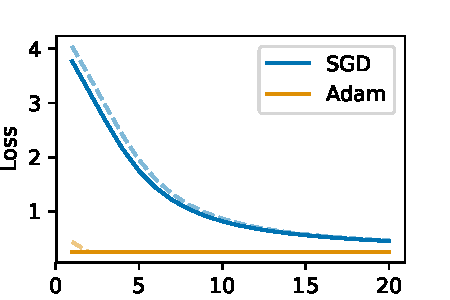
\includegraphics[width=.6\textwidth]{./Chapter_network_fusion/cerevisiae/deepNF/180809_d7d6015/cerevisiae_MDA_arch_2000-600_optimizers}
%     \caption{%Optimisers: MDAE reconstruction loss. Comparing MDAE reconstruction loss for MDAs trained using SGD (\emph{blue}) and Adam (\emph{orange}). \losscerevisiae{2000-600}}
%     \label{fig:sgd-vs-adam-loss}
% \end{figure}
%
% \begin{figure}[!ht]
%     \centering
%     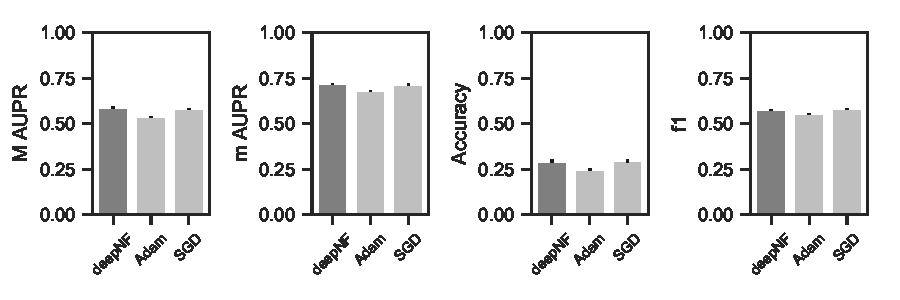
\includegraphics{./Chapter_network_fusion/cerevisiae/classification/cv_cerevisiae_level1_MDA-2000-600-optimizers}
%     \caption{%Optimisers: cross-validation results. Cross-validation performance using embeddings generated by an MDAE using SGD (\emph{blue}) and Adam (\emph{orange}). \cvmipssvm\ \cvlevelone\ \cvdeepnfcomparison}
%     \label{fig:sgd-vs-adam-cv}
% \end{figure}
%
% \paragraph{Conclusion}\label{conclusion}
%
% These experiments compared the effects of replacing techniques used in deepNF with current best practices for neural networks. Whilst ReLU and Adam result in MDAs with lower validation loss and faster convergence, the prediction performance of SVMs trained on protein embeddings from these models is lower. This result is counterintuitive and I cannot explain it. One would expect a lower MDAE loss to be correlated with improved prediction performance, however, this trend is not apparent. A note in the supplementary information of the deepNF paper confirms the findings about the activation function:
%
% \begin{quote}
% ``We have tried a variety of activation functions including tanh and ReLU, and have found empirically that the sigmoid activation performed the best.''
% \end{quote}
%
% Another note claims that the choice of optimiser has little effect:
%
% \begin{quote}
% ``Optimizers such as Adam and Adagrad seemed not to have much of an effect on final performance of our models, so for simplicity we chose to train our models using stochastic gradient descent with momentum.''
% \end{quote}
%
% However, I find that there is a significant reduction in performance when Adam is used instead of SGD.

\subsection{Small embeddings achieve comparable performance to deepNF}
\label{sec:experiment-with-different-mda-architectures}


%many training examples as there are proteins in \emph{S. cerevisiae} and \emph{S. pombe}, we should use smaller architectures.

It is advantageous to use the smallest MDAE architecture---with the fewest number of layers, neurons and embedding dimensions---to reduce the training time of both the MDAE and classifier.
However, there is no \emph{a priori} way to choose the best neural network architecture.
Instead, a variety of different architectures should be tested according to
the following rules of thumb:

\begin{itemize}
    \item Due to the layout of memory on the GPU, neural networks are trained best when using a power of $2$ number of neurons in each layer (e.g. $128$, $256$, $512$ and $1024$).
    % We trained a variety of MDAs consisting of two to four layers in the encoding portion, with layer sizes varying from 128 to 1024.
    \item The output of a preceeding layer should always used as input to a layer of the same, or smaller, size (e.g. $512 \rightarrow 512 \rightarrow 128$). In autoencoders, this rule should only be applied to the encoding part of the network; decoders are the mirror image of the encoder.
    %(Note that this is not the case in the decoding portion of the MDAE.)
\end{itemize}

% I replaced two outdated techniques that deepNF used in the MDAE with current best practices for neural networks in an attempt to improve prediction performance (\ref{table:best-practices-overview}).
%
% \begin{table}[!ht]
%     \centering
%     \caption{%Best practices: improving deepNF with current best practices.}
%     \label{table:best-practices-overview}
%     \begin{tabularx}{\textwidth}{lllX}
%         \toprule
%         & \textbf{deepNF} & \textbf{Replacement} & \textbf{Explanation} \\
%         \midrule
%         \textbf{Activation function} & Sigmoid & ReLU & Overcomes the problems of vanishing gradients associated with sigmoid activations, that squash the entire number line into the interval $[0,1]$ \\
%         \textbf{Optimiser} & SGD & Adam & More recent optimisers find the optimal direction and magnitude with which to update weights, allowing neural networks to train and converge faster \\
%         \bottomrule
%     \end{tabularx}
% \end{table}



% \subsubsection{Estimating the number of epochs required to train an MDAE}\label{estimating-the-number-of-epochs-required-to-train-an-mda}

To estimate the number of epochs required to train smaller MDAE architectures, we trained an arbitrary $512$-$128$ MDAE architecture for $2000$ epochs.
Training for $500$ epochs is sufficient because the MDAE started overfitting on the training data after $\sim 150$ epochs.
Going forward, we train MDAs for $500$ epochs and save weights from the epoch with the lowest validation loss.

% was chosen to estimate the number of epochs required for training (\ref{table:estimating-epochs}). Training for 500 epochs is sufficient for this (and larger) architectures, as the MDAE is clearly overfitting on the training data after \textasciitilde{}150 epochs. The loss for the best epoch (0.166 after 121 epochs) is lower than the best loss for the 2000-600 MDAE using Adam and ReLU. Going forward, I train MDAs for 500 epochs and save weights from the epoch with the lowest validation loss.

% \begin{table}[!ht]
%     \centering
%     \caption{%MDAE parameters for estimating the number of epochs required to train an MDAE.}
%     \label{table:estimating-epochs}
%     \begin{tabular}{ll}
%         \toprule
%         \textbf{Parameter} & \textbf{Value} \\
%         \midrule
%         MDAE architecture & 512-128 \\
%         Activation function & ReLU \\
%         Optimiser & Adam \\
%         Epochs & 2000 \\
%         \bottomrule
%     \end{tabular}
% \end{table}

% \begin{figure}[!ht]
%     \centering
%     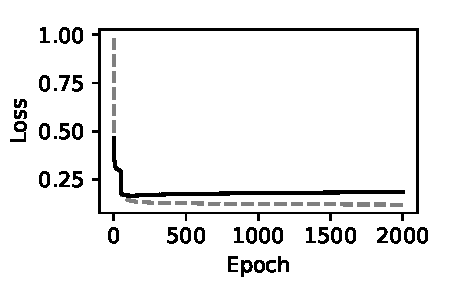
\includegraphics[width=.6\textwidth]{./Chapter_network_fusion/cerevisiae/autoencoder/architectures_relu_2000_epochs}
%     \caption{%Estimating the number of epochs required to train a low-dimensional MDAE. \losscerevisiae{512-128}}
%     \label{fig:estimating-epochs-loss}
% \end{figure}

% \subsubsection{Compare 128D and 256D embeddings generated by different MDAE architectures}\label{compare-128d-and-256d-embeddings-generated-by-different-mda-architectures}

We trained nine different MDAE architectures that embed proteins into a $128$D or $256$D space. \mdaarchitectures\ The $256$-$256$ MDAE had the lowest validation loss of $0.162$ after $161$ epochs (\ref{fig:compare-architectures-loss}). Embeddings from this MDAE were taken forward for further experiments.
%used in subsequent experiments were generated by the 256-256 MDAE.

% \begin{table}[!ht]
%     \centering
%     \caption{%MDAE parameters for comparing 128D and 256D embeddings generated by different MDAE architectures.}
%     \label{table:compare-architectures}
%     \begin{tabular}{ll}
%         \toprule
%         \textbf{Parameter} & \textbf{Value} \\
%         \midrule
%         MDAE architecture & Various \\
%         Activation function & ReLU \\
%         Optimiser & Adam \\
%         Epochs & 2000 \\
%         \bottomrule
%     \end{tabular}
% \end{table}

\begin{figure}[!hbt]
    \centering
    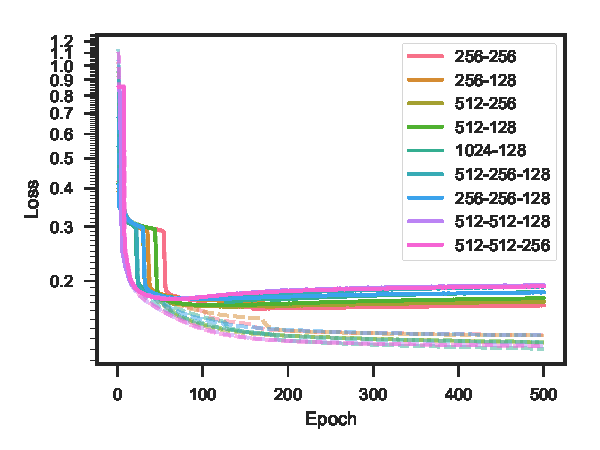
\includegraphics[width=\textwidth]{./Chapter_network_fusion/cerevisiae/autoencoder/architectures_relu}
    \caption{%
        \emph{S. cerevisiae} MDAE reconstruction losses for different MDAE architectures that produce $128$D and $256$D embeddings.
        Binary crossentropy loss on the validation set is plotted.
        % \mdaarchitectures\
        % MDAs were trained on \emph{S. cerevisiae} data derived from six STRING networks and used to generate protein embeddings.
        % The reconstruction loss was calculated on a validation set consisting of $10\%$ of the available data.
    }
    \label{fig:compare-architectures-loss}
\end{figure}

% \subsubsection{Benchmark low dimensional embeddings using deepNF's SVMs}\label{benchmark-low-dimensional-embeddings-using-deepnfs-svms}

We benchmarked the predictive performance of these embeddings, using the same supervised machine learning procedure used by deepNF.
We found that the $256$D embeddings have an equivalent performance to the $600$D embeddings used by deepNF (\ref{fig:256D-embeddings-SVM-cv}).
This is a significant improvement over deepNF because smaller MDAs have fewer parameters to train,
they are less likely to be underfit on small training data sets,
and they can be trained much faster.
Finally, SVM training time will be faster on smaller embeddings.


%     \item Less likely to overfit on a smaller number of training examples
%     \item Trains much faster
%     \item There are fewer non-informative dimensions
%     \item SVMs can be trained much faster as there are fewer features
% \end{itemize}

 % generated by the 2000-600 MDAE


% the 256D protein embeddings generated by the 256-256 MDAE using the same prediction procedure used by deepNF (\ref{fig:256D-embeddings-SVM-cv}). These results show that the 256D embeddings are equivalent to the 600D embeddings generated by the 2000-600 MDAE. This is a significant improvement over deepNF for a number of reasons:
%
% \begin{itemize}
%     \item The 256-256 MDAE has fewer parameters to train
%     \item Less likely to overfit on a smaller number of training examples
%     \item Trains much faster
%     \item There are fewer non-informative dimensions
%     \item SVMs can be trained much faster as there are fewer features
% \end{itemize}

\begin{figure}[!hbt]
    \centering
    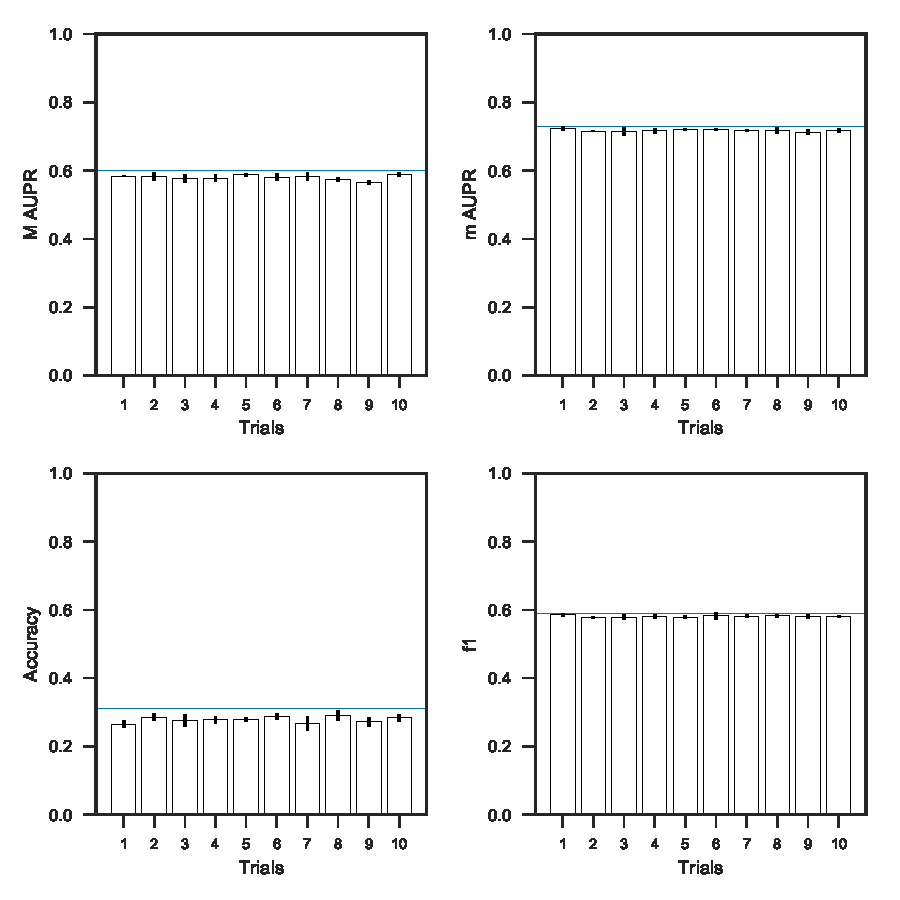
\includegraphics[width=\textwidth]{./Chapter_network_fusion/cerevisiae/classification/cv_cerevisiae_level1_MDA-256-256-ReLU-deepNF-SVM}
    \caption{%
        \emph{S. cerevisiae} protein function prediction performance on $256$D embeddings.
        SVMs were trained to predict MIPS terms in the one-vs-rest strategy.
        MIPS terms were divided into three levels according to the number of proteins that are annotated with each term.
        Results for level 1 terms are plotted (light grey bars).
        deepNF results from \ref{fig:replicate-deepNF-cv} are shown for comparison (dark grey bars).
        Bars are the mean performance across $10$ independent trials of $5$-fold cross-validation and error bars are the standard deviation.
        % Cross-validation results using low-dimensional embeddings.
        % The embeddings produced by a 256-256 MDAE were used as these had the lowest reconstruction loss.
        % Protein embeddings were used as features to train a one-vs-rest SVM to predict MIPS annotations.
        % MIPS terms were divided into three levels according to the number of proteins that are annotated with each term: 101-300 proteins in level 1, 31-100 proteins in level 2, and 11-30 proteins in level 3. 10 independent trials of 5-fold cross-validation were performed. The mean performance across the independent trials is shown. Error bars show the standard deviation.
        % Results for level 1 terms are shown.
        % deepNF results from \ref{fig:replicate-deepNF-cv} are shown for comparison.
    }
    \label{fig:256D-embeddings-SVM-cv}
\end{figure}

\subsection{Sets of protein functions can be predicted simultaneously using structured learning}
\label{structured-prediction-of-mips-annotations}

Using our $256$D embeddings, we saught to improve on the performance of deepNF.
To do this, we trained neural networks instead of SVMs.
Whilst most classifiers output a scalar value, neural networks output a vector.
The output vector can predict all classes of a multiclass prediction task simultaneously, in a supervised learning paradigm called structured learning or structured prediction.
In this paradigm, a model can be learnt to predict multiple classes that are not mutually exclusive, whilst simultaneously learning non-linear correlations between features and labels.
Output vectors can be converted to probabilities by applying the softmax function
\[
S(x_i) = \frac{e^{x_i}}{\sum_j e^{y_j}}.
\]

%For the remainder of this chapter, I train MLPs using structured learning to predict vectors of MIPS terms for \emph{S. cerevisiae} and GO terms for \emph{S. pombe}.
% This architecture is able to be trained with the protein embeddings and provides good performance. Two parameters---the dropout rate and batch size---need to be chosen empirically, which I outline below.
%
% \paragraph{Dropout}\label{dropout}
%
% Dropout regularization was applied to the output of the 512 neuron hidden layer with probabilities $\{0, 0.25, 0.5\}$ and benchmarked by 10 independent trials of 5-fold cross-validation (\ref{fig:dropout}). For some metrics, the structured learning performance matches deepNF, whilst in other metrics, the performance is worse. A dropout rate of 0.5 generally yields the highest performance, so was used in subsequent experiments.
%
% \begin{figure}[!ht]
%     \centering
%     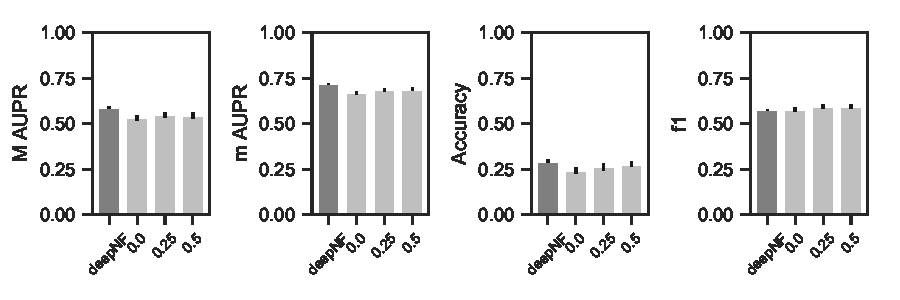
\includegraphics{./Chapter_network_fusion/cerevisiae/mlp/cv_cerevisiae_level1_MDA-256-256-ReLU_MLP}
%     \caption{%Dropout: structured prediction cross-validation results. The effect of the dropout rate was tested. protein embeddings from a 256-256 MDAE were used as features to train 512-256 MLPs with p(dropout) of 0, 0.25 or 0.5. \cvmipsmlp\ \cvlevelone\ \cvdeepnfcomparison}
%     \label{fig:dropout}
% \end{figure}

% \paragraph{Batch size}\label{batch-size}
%
% The batch size (number of training examples processed per batch) must be assessed. Powers of two batch sizes are most efficient, due to GPU vectorisation. I tested batch sizes of 64, 128, 256, 512 and 1024 examples (\ref{fig:batch-size}). No single batch size is best for all three levels of annotations and 128 appears to be the best compromise. For some metrics, the structured learning performance matches deepNF, whilst in other metrics, the performance is worse.
%
% \begin{figure}[!ht]
%     \centering
%     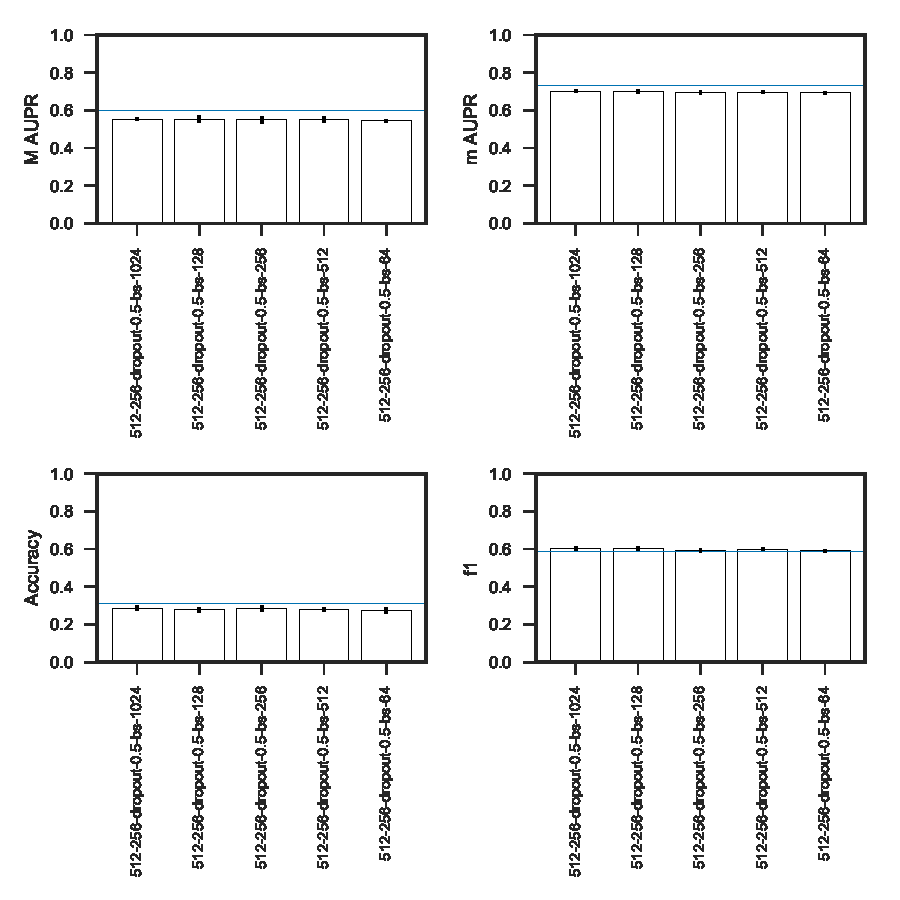
\includegraphics{./Chapter_network_fusion/cerevisiae/mlp/cv_cerevisiae_level1_MDA-256-256-ReLU_MLP_batch-size}
%     \caption{%Batch size: structured prediction cross-validation results. The effect of the batch size was tested. protein embeddings from a 256-256 MDAE were used as features to train 512-256 MLPs with 0.5 dropout and batch sizes of 64, 128, 256, 512 and 1024. \cvmipsmlp\ \cvlevelone\ \cvdeepnfcomparison}
%     \label{fig:batch-size}
% \end{figure}

% \subsubsection{Train MDAE on unprocessed STRING adjacency matrices}\label{train-mda-on-unprocessed-string-adjacency-matrices}
%
% deepNF processed the STRING adjacency matrices by Cao's method \cite{Cao2016} using RWR, to reduce the sparsity of the graph, and by PPMI, to remove redundant edges. The random walks, however, introduce undesirable stochasticity into the method. Ideally, we want a deterministic input to the MDAE. (MDAs and MLPs are inherently stochastic, but these models tend to approximately converge to the global optimum, or a good local optimum.)
%
% To test whether the adjacency matrices need to be processed with RWR and PPMI, I trained a variety of MDAE architectures on unprocessed adjacency matrices (\ref{fig:raw-loss}). Some architectures achieve a validation loss of \textasciitilde{}0.05 after 60-90 epochs, which is much lower than the loss achievable when using processed adjacency matrices. Some wide architectures---consisting of layers with 512 or 1024 neurons, or deep architectures with 3 hidden layers in the encoding portion---do not learn. The best architecture is 512-256 MDAE with a validation loss of 0.051. The embeddings from the best epoch of this MDAE were benchmarked using an MLP (\ref{fig:raw-cv}). The performance is significantly worse than the published performance of deepNF, so RWR and PPMI are indeed necessary for performance.
%
% \begin{figure}[!ht]
%     \centering
%     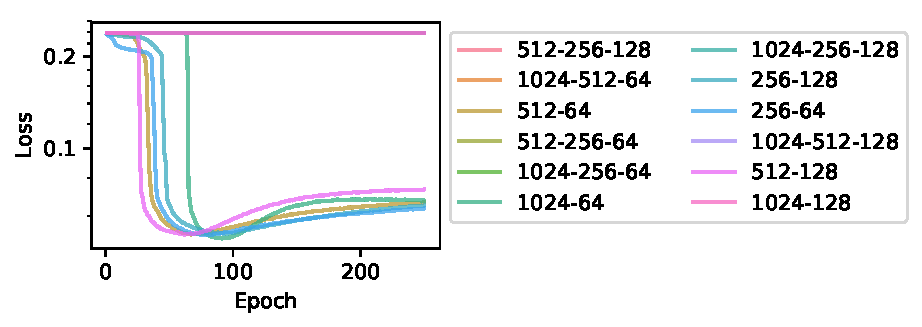
\includegraphics{./Chapter_network_fusion/cerevisiae/autoencoder/architectures_no_rwr_ppmi_64D_128D}
%     \caption{%Raw STRING adjacency matrices: reconstruction loss. Losses for different MDAE architectures producing 128D and 256D embeddings trained on raw STRING adjacency matrices. MDAs were trained on \emph{S. cerevisiae} data derived from 6 STRING networks, whose adjacency matrices were not pre-processed with RWR or PPMI. 128D embeddings were generated by 256-128, 512-128, 1024-128, 512-256-128, 1024-256-128 and 1024-512-128 MDAE architectures. 64D embeddings were generated by 256-64, 512-64, 1024-64, 512-256-64, 1024-256-64 and 1024-512-64 MDAE architectures. MDAs were \losscerevisiaetext}
%     \label{fig:raw-loss}
% \end{figure}
%
% \begin{figure}[!ht]
%     \centering
%     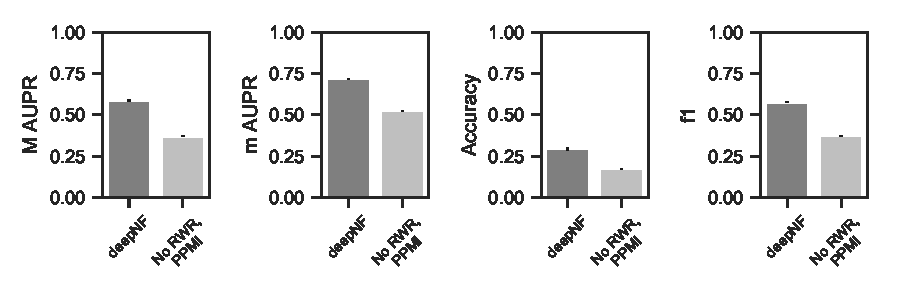
\includegraphics{./Chapter_network_fusion/cerevisiae/mlp/cv_cerevisiae_level1_no_RWR_PPMI}
%     \caption{%Raw STRING adjacency matrices: structured prediction cross-validation results. 256D protein embeddings from a 512-256 MDAE trained on raw STRING adjacency matrices were used as features to train a 512-256 MLP with 0.5 dropout to predict all MIPS terms in a level simultaneously. \cvmipsmlp\ \cvlevelone\ \cvdeepnfcomparison}
%     \label{fig:raw-cv}
% \end{figure}

% \subsubsection{Final predictions of protein function}\label{final-predictions}

After much experimentation, we settled on an MLP with two hidden layers of $512$ and $256$ neurons, a dropout probability of $0.5$ and a batch size of $128$.
% Concluding my work on \emph{S. cerevisiae}, I integrated my findings to make high-quality protein function predictions. Using the best 256D embeddings from a 256-256 MDAE, I trained a 512-256 MLP with a 0.5 dropout rate and benchmarked these predictions against the published metrics for deepNF
The structured prediction performance of the MLP is comparable with deepNF's one-vs-rest SVM predictions (\ref{fig:levels-cerevisiae-cv}).
% The structured prediction performance is comparable with the one-vs-rest SVM predictions.
Whilst the MLP has slightly lower performance according to mAUPR, MAUPR and accuracy, their f1 performance is higher.
On balance, we believe that these moderate reductions in performance are worthwhile, due to the concomitant benefits of structured prediction and the orders of magnitude faster training time compared to one-vs-rest SVMs.

\begin{figure}[!hbt]
    \centering
    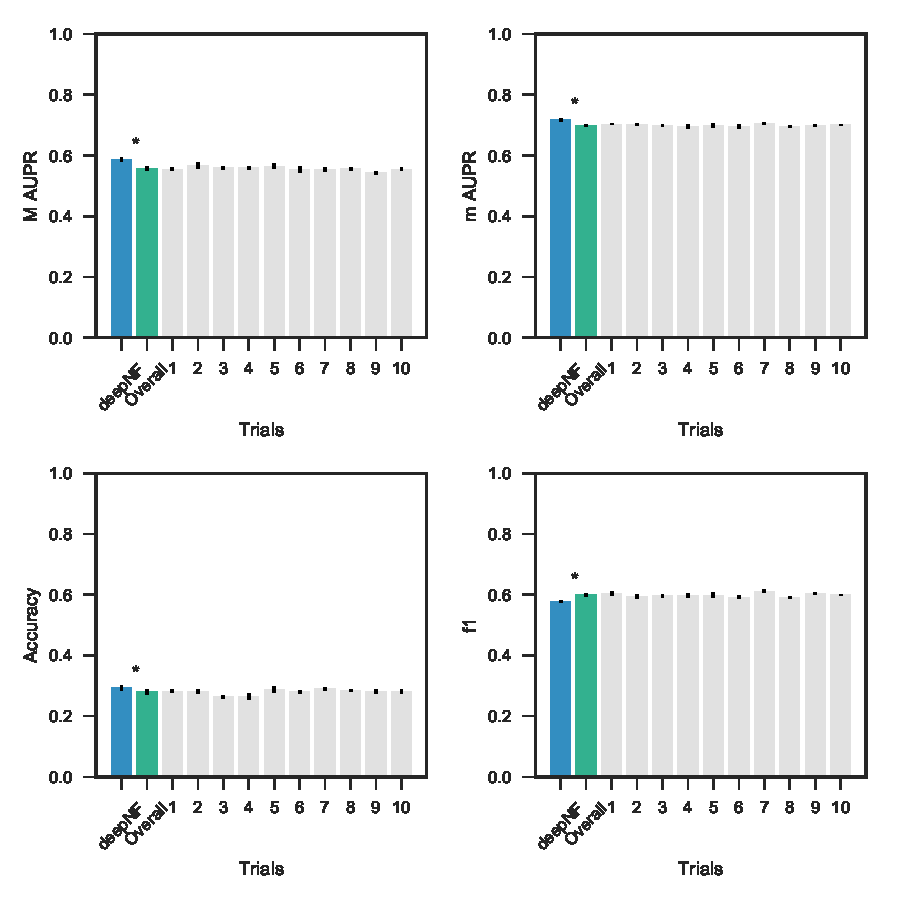
\includegraphics[width=\textwidth]{./Chapter_network_fusion/cerevisiae/mlp/cv_cerevisiae_level1_MDA-256-256-MLP-512-256}
    \caption{%
        \emph{S. cerevisiae} protein function prediction performance using structured learning on $256$D embeddings.
        MLPs were trained to predict all MIPS terms in a level simultaneously.
        MIPS terms were divided into three levels according to the number of proteins that are annotated with each term.
        Results for level 1 terms are plotted (light grey bars).
        deepNF results from \ref{fig:replicate-deepNF-cv} are shown for comparison (dark grey bars).
        Bars are the mean performance across $10$ independent trials of $5$-fold cross-validation and error bars are the standard deviation.
        % Structured prediction cross-validation results.
        % $256$D protein embeddings from a $512$-$256$ MDAE were used as features to train a $512$-$256$ MLP with $0.5$ dropout to predict all MIPS terms in a level simultaneously.
        % Protein embeddings were used as features to train an MLP to predict MIPS annotations.
        % MIPS terms were divided into three levels according to the number of proteins that are annotated with each term: 101-$300$ proteins in level 1, 31-100 proteins in level 2, and 11-30 proteins in level 3. 10 independent trials of 5-fold cross-validation were performed. The mean performance across the independent trials is shown. Error bars show the standard deviation.
        % Results for level 1 terms are shown.
        % deepNF results from \ref{fig:replicate-deepNF-cv} are shown for comparison.
    }
    \label{fig:levels-cerevisiae-cv}
\end{figure}

% \subsubsection{Prediction of all annotations at once}\label{predicting-all-annotations-at-once}
%
% Additionally, I tried predicting all 244 MIPS annotations simultaneously by pooling terms from the three levels (\ref{fig:all-cerevisiae-cv}). With the exception of accuracy---which is an extremely tough metric for multiclass predictions---I am able to predict all annotations approximately as well as deepNF predicts the hardest level 3 terms (orange line). Predicting a 244-element vector is rather a difficult task, so it is not surprising that the performance is as on par with the published performance for level 3. The MLP may have learnt correlations between terms to make correct novel predictions, but the only way to know is to validate predictions experimentally.
%
% \begin{figure}[!ht]
%     \centering
%     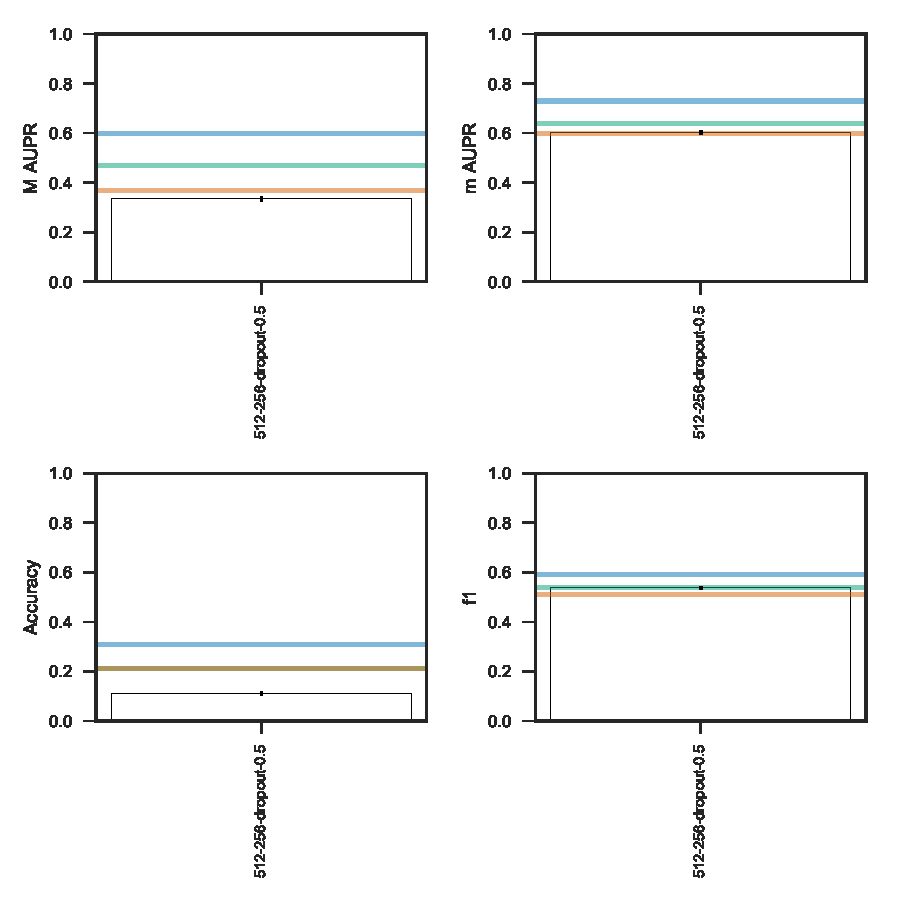
\includegraphics{./Chapter_network_fusion/cerevisiae/mlp/cv_cerevisiae_all_MLP-512-256}
%     \caption{%Structured prediction cross-validation results. 256D protein embeddings from a 512-256 MDAE were used as features to train a 512-256 MLP with 0.5 dropout to predict all MIPS terms simultaneously. \cvmipstext\ \cvdeepnfcomparison}
%     \label{fig:all-cerevisiae-cv}
% \end{figure}


\subsection{Embeddings of yeast proteins predict function}
\label{sec:results-pombe}

% Having thoroughly investigated various ways to improve deepNF using \emph{S. cerevisiae} data, I next moved to using \emph{S. pombe} data to predict GO term annotations.

% \subsubsection{Analysis of \emph{S. pombe} protein Ontology annotations}
%
% The quality of \emph{S. pombe} GO annotations was analysed by plotting the distribution of proteins annotated with terms from different evidence code classes. The classes were `experimental', `computational', `curated' and `automatic'--in descending order of quality. The number of proteins with at least one annotation from an evidence code class is shown in \ref{fig:pombe-go-analysis}. Note that a protein annotated with many computational, curated and automatic terms, but a single experimental term, will be contained in the experimental class of the stacked bar plot. The same is true for each of computational and curated classes.
%
% \emph{S. pombe} has been studied experimentally extensively. In comparison to other species, many of its proteins have at least one experimental GO annotation. Approximately one third of proteins have experimental annotations from the biological process or molecular function ontologies. About three times as many proteins have experimental annotations from the
% cellular componenet ontology. More than one third of proteins have computational annotations from the biological process or molecular function ontologies. The large number of these annotations may have been inherited from related species of yeast, including \emph{S. cerevisiae}, which has been extensively studied experimentally. Later, I discuss whether there is any correlation between the quality of annotations and the ability to predict GO terms per ontology.
%
% \begin{figure}[!ht]
%     \centering
%     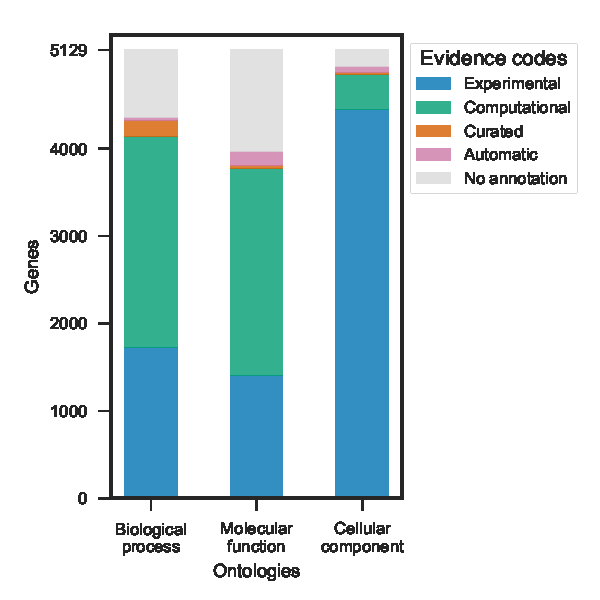
\includegraphics[width=.6\textwidth]{./Chapter_network_fusion/pombe/evidence_codes_of_gene_annotations}
%     \caption{%Analysis of the \emph{S. pombe} GO annotations.}
%     \label{fig:pombe-go-analysis}
% \end{figure}

% \subsubsection{Generate protein embeddings}\label{generate-gene-embeddings}
With a performant protein function prediction model in hand, we next focussed our attention on predicting \emph{S. pombe} protein functions.
First, we generated embeddings for the $5100$ \emph{S. pombe} proteins contained in STRING (v10.5), using the same MDAE architectures as \emph{S. cerevisiae}. Similar to \emph{S. cerevisiae}, we found that the $256$-$256$ MDAE was the best architecture, achieving a validation loss of $0.221$ after $127$ epochs.
% (\ref{fig:pombe-loss}). I used the same MDAE architectures as were used for \emph{S. cerevisiae} and found that 256-256 MDAE was also the best architecture for \emph{S. pombe}, achieving a validation loss of 0.221 after 127 epochs.
Validation losses were much higher for \emph{S. pombe} than for \emph{S. cerevisiae}, which may reflect the higher sparsity of \emph{S. pombe} data, compared with \emph{S. cerevisiae}, which has been studied extensively.

%
% \begin{figure}[!ht]
%     \centering
%     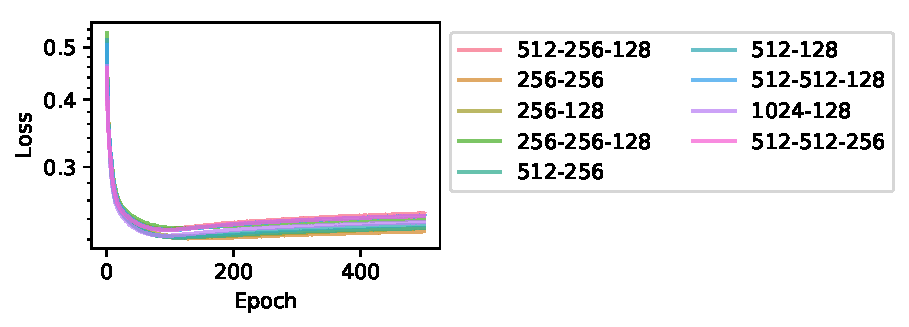
\includegraphics{./Chapter_network_fusion/pombe/autoencoder/architectures_6-networks}
%     \caption{%Losses for different MDAE architectures producing 128D and 256D embeddings. \mdaarchitectures\ MDAs were \losspombetext}
%     \label{fig:pombe-loss}
% \end{figure}

% \subsubsection{Structured prediction of terms from three levels of each ontology}\label{structured-prediction-of-terms-from-three-levels-of-each-ontology}

Using the $256$D embeddings, we predicted GO term annotations from each ontology using a $512$-$256$ MLP and structured learning (\ref{fig:pombe-levels-cv}).
We achieved good performance for predicting functions of proteins from level 1 for all ontologies.
Level 2 terms were also predicted well according mAUPR, MAUPR and f1, but not according to accuracy.
In this case, the subset accuracy is a harsh metric for multiclass prediction because the vector of predictions must exactly match the vector of labels.
Biological process and molecular function terms were predicted less well than cellular component terms in level 3.
Overall, the performance of predicting terms from the cellular component ontology is more consistent across the three levels.
% With respect to the quality of annotations per ontology \ref{fig:pombe-go-analysis}, there may be a correlation between the number of proteins with experimental annotations and the performance of predicting GO terms.


\begin{figure}[!hbt]
    \centering
    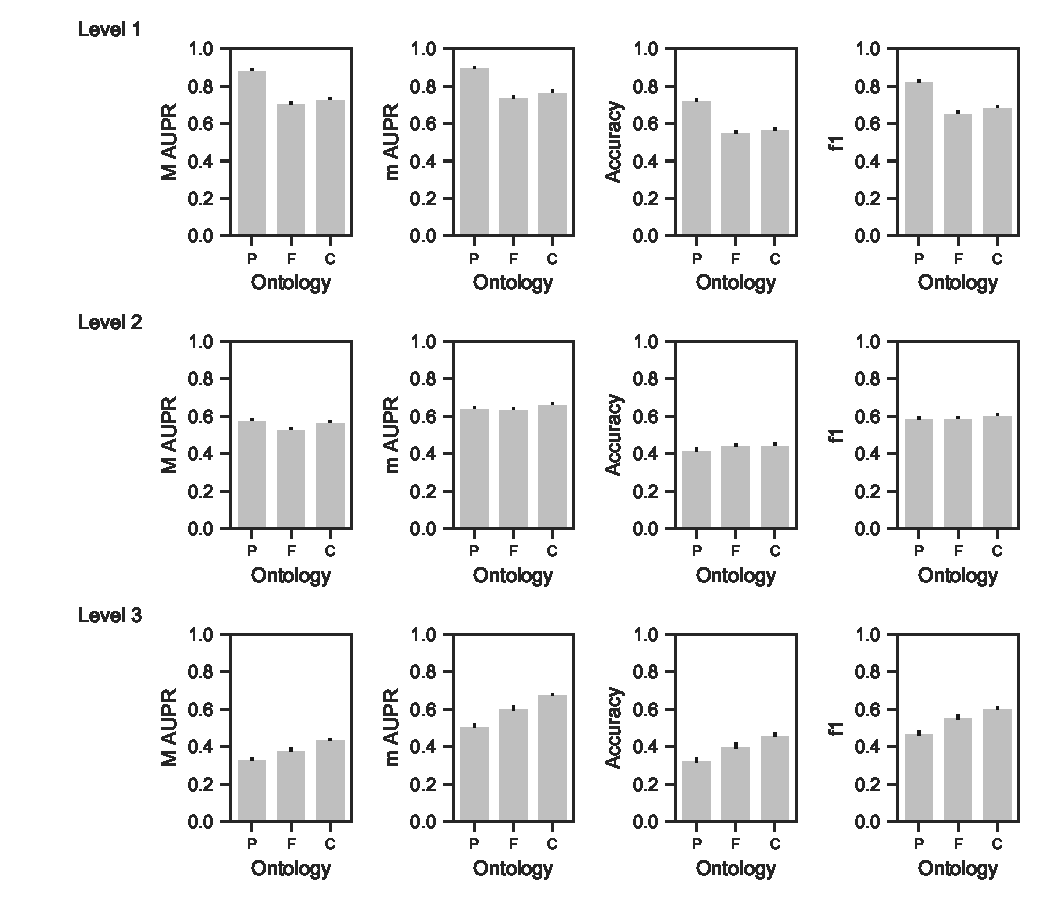
\includegraphics[width=\textwidth]{./Chapter_network_fusion/pombe/mlp/cv_pombe_PFC_separate_MLP-512-256}
    \caption{%
        \emph{S. pombe} protein function prediction performance using structured learning on $256$D embeddings.
        MLPs were trained to predict all GO terms in a level simultaneously.
        GO terms were divided into three levels according to the number of proteins that are annotated with each term.
        Bars are the mean performance across $10$ independent trials of $5$-fold cross-validation and error bars are the standard deviation.
        % Structured prediction of GO annotations for each ontology divided into three levels.
        % All GO terms from an ontology and level were predicted simultaneously.
        % 256D protein embeddings from a 256-256 MDAE were used as features to train a 512-256 MLP with 0.5 dropout to predict all GO terms in a level simultaneously from the biological process (P), molecular function (F) and cellular component (C) ontologies.
        % GO terms from each ontology were divided into three levels according to the number of proteins that are annotated with each term: 101-300 proteins in level 1, 31-100 proteins in level 2, and 11-30 proteins in level 3. 10 independent trials of 5-fold cross-validation were performed. The mean performance across the independent trials is shown. Error bars show the standard deviation.
    }
    \label{fig:pombe-levels-cv}
\end{figure}



% \subsubsection{Structured prediction of terms from each ontology}\label{structured-prediction-of-terms-from-each-ontology}

Splitting terms into three levels according to how many proteins they are annotated to seems quite arbitrary. Instead, we trained models to predict all terms from an ontology simultaneously using structured learning (\ref{fig:pombe-all-cv}).
Generally speaking, we are able to predict all terms in an ontology with approximately the same performance of predicting level 3 terms in \ref{fig:pombe-levels-cv}.
Whilst these trends are true for mAUPR, MAUPR and f1, it is not true for accuracy, due to a subset accuracy of $\sim 0.25$ for each ontology.

% For the biological process ontology, the performance is slightly higher than for level 3 terms (\ref{fig:pombe-levels-cv}) for the metrics MAUPR, mAUPR and f1.
% For the molecular function ontology, mAUPR and f1 are higher in level 3 than when the entire ontology is predicted, but MAUPR is approximately the same. All metrics are higher for level 3 of the cellular component ontology than when the entire ontology is predicted.


% (Subset) accuracy is an extremely harsh metric in the multiclass prediction, as the entire predicted vector must match the known labels. It's no wonder that the accuracy is \textasciitilde{}0.25 for each ontology when predicting vectors of length XYZ-ABC.

\begin{figure}[!hbt]
    \centering
    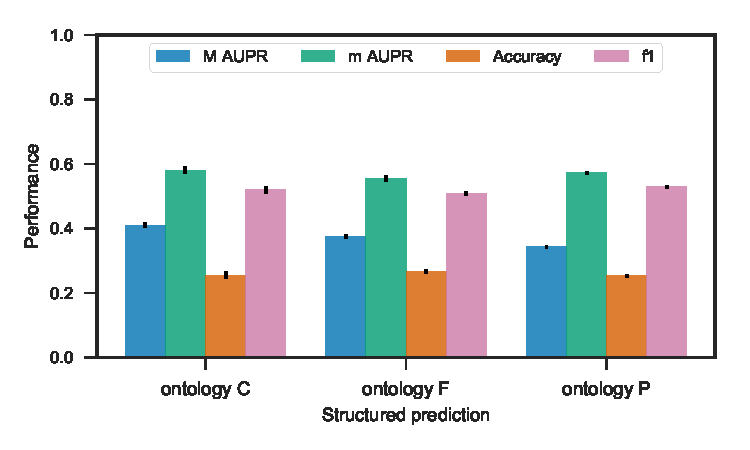
\includegraphics[width=\textwidth]{./Chapter_network_fusion/pombe/mlp/cv_pombe_structured}
    \caption{%
        \emph{S. pombe} protein function prediction performance using structured learning on $256$D embeddings.
        MLPs were trained to predict all GO terms in an ontology simultaneously.
        Bars are the mean performance across $10$ independent trials of $5$-fold cross-validation and error bars are the standard deviation.
        % Structured prediction of GO annotations for each ontology.
        % All GO terms from an ontology were predicted simultaneously.
        % 256D protein embeddings from a 256-256 MDAE were used as features to train a 512-256 MLP with 0.5 dropout to predict all GO terms in a level simultaneously from the biological process (P), molecular function (F) and cellular component (C) ontologies.
        % GO terms from each ontology were divided into three levels according to the number of proteins that are annotated with each term: 101-300 proteins in level 1, 31-100 proteins in level 2, and 11-30 proteins in level 3. 10 independent trials of 5-fold cross-validation were performed. The mean performance across the independent trials is shown. Error bars show the standard deviation.
    }
    \label{fig:pombe-all-cv}
\end{figure}


\subsection{Including orthogonal protein network data did not increase prediction performance}
\label{incorporating-additional-data-modes}

In order to learn a low-dimensional embeddings space, MDAs perform data fusion of multple networks. The goal of data fusion is to combine multiple, heterogenous and orthogonal data sets together into a composite data set, whose predictive power is higher than any one data set alone. deepNF fused six types of protein network data encoded in the STRING database. Many more types of interactions between proteins are possible, but were not included in deepNF. Here, we tested whether the predictive power of protein embeddings could be increased by including other, orthogonal types of interactions:

\begin{itemize}
    \item genetic interactions from the BioGRID database,
    \item gene co-expression correlations from a meta-analysis of \emph{S. pombe} protein expression studies \cite{Pancaldi2010}, and
    \item experimental phenotypes from the fission yeast phenotype ontology.
\end{itemize}

We fused these three networks and the six STRING networks using the same set of MDAE architectures that we used in \ref{sec:results-pombe}.
% (\ref{fig:pombe-9-networks-loss}).
The $256$-$256$ MDAE architecture had the best validation loss of $0.403$. For comparison, this loss is much higher than the best loss of $0.221$ when autoencoding the six STRING networks (\ref{sec:results-pombe}). This suggests that the three additional networks are noisy,
% add a significant amount of noise that
reducing the MDAE's ability to reconstruct the networks.
An alternative argument to explain this result could be that the reconstruction loss is higher for nine input networks because the $256$-$256$ MDAE's neurons were saturated and the MDAE has reached its maximum reconstruction capacity.
However, this situation is unlikely to be true because $31$ embedding dimensions remain untrained in the MDAE, where all values in these dimensions are zero for all proteins.
Also, other architectures that were larger, such as the $512$-$512$-$256$ MDAE, had very similar loss curves.
Either way, the $256$D embeddings generated by feature learning from nine networks had a lower prediction performance (\ref{fig:pombe-9-networks-cv}) than $256$D embeddings from six STRING networks (\ref{fig:pombe-levels-cv}).

% \begin{figure}[!ht]
%     \centering
%     % NB code to produce this figure is in:
%     % $POMBEAGEINGGENES/Scripts/network_embeddings/plot_clusteredheatmaps.py
%     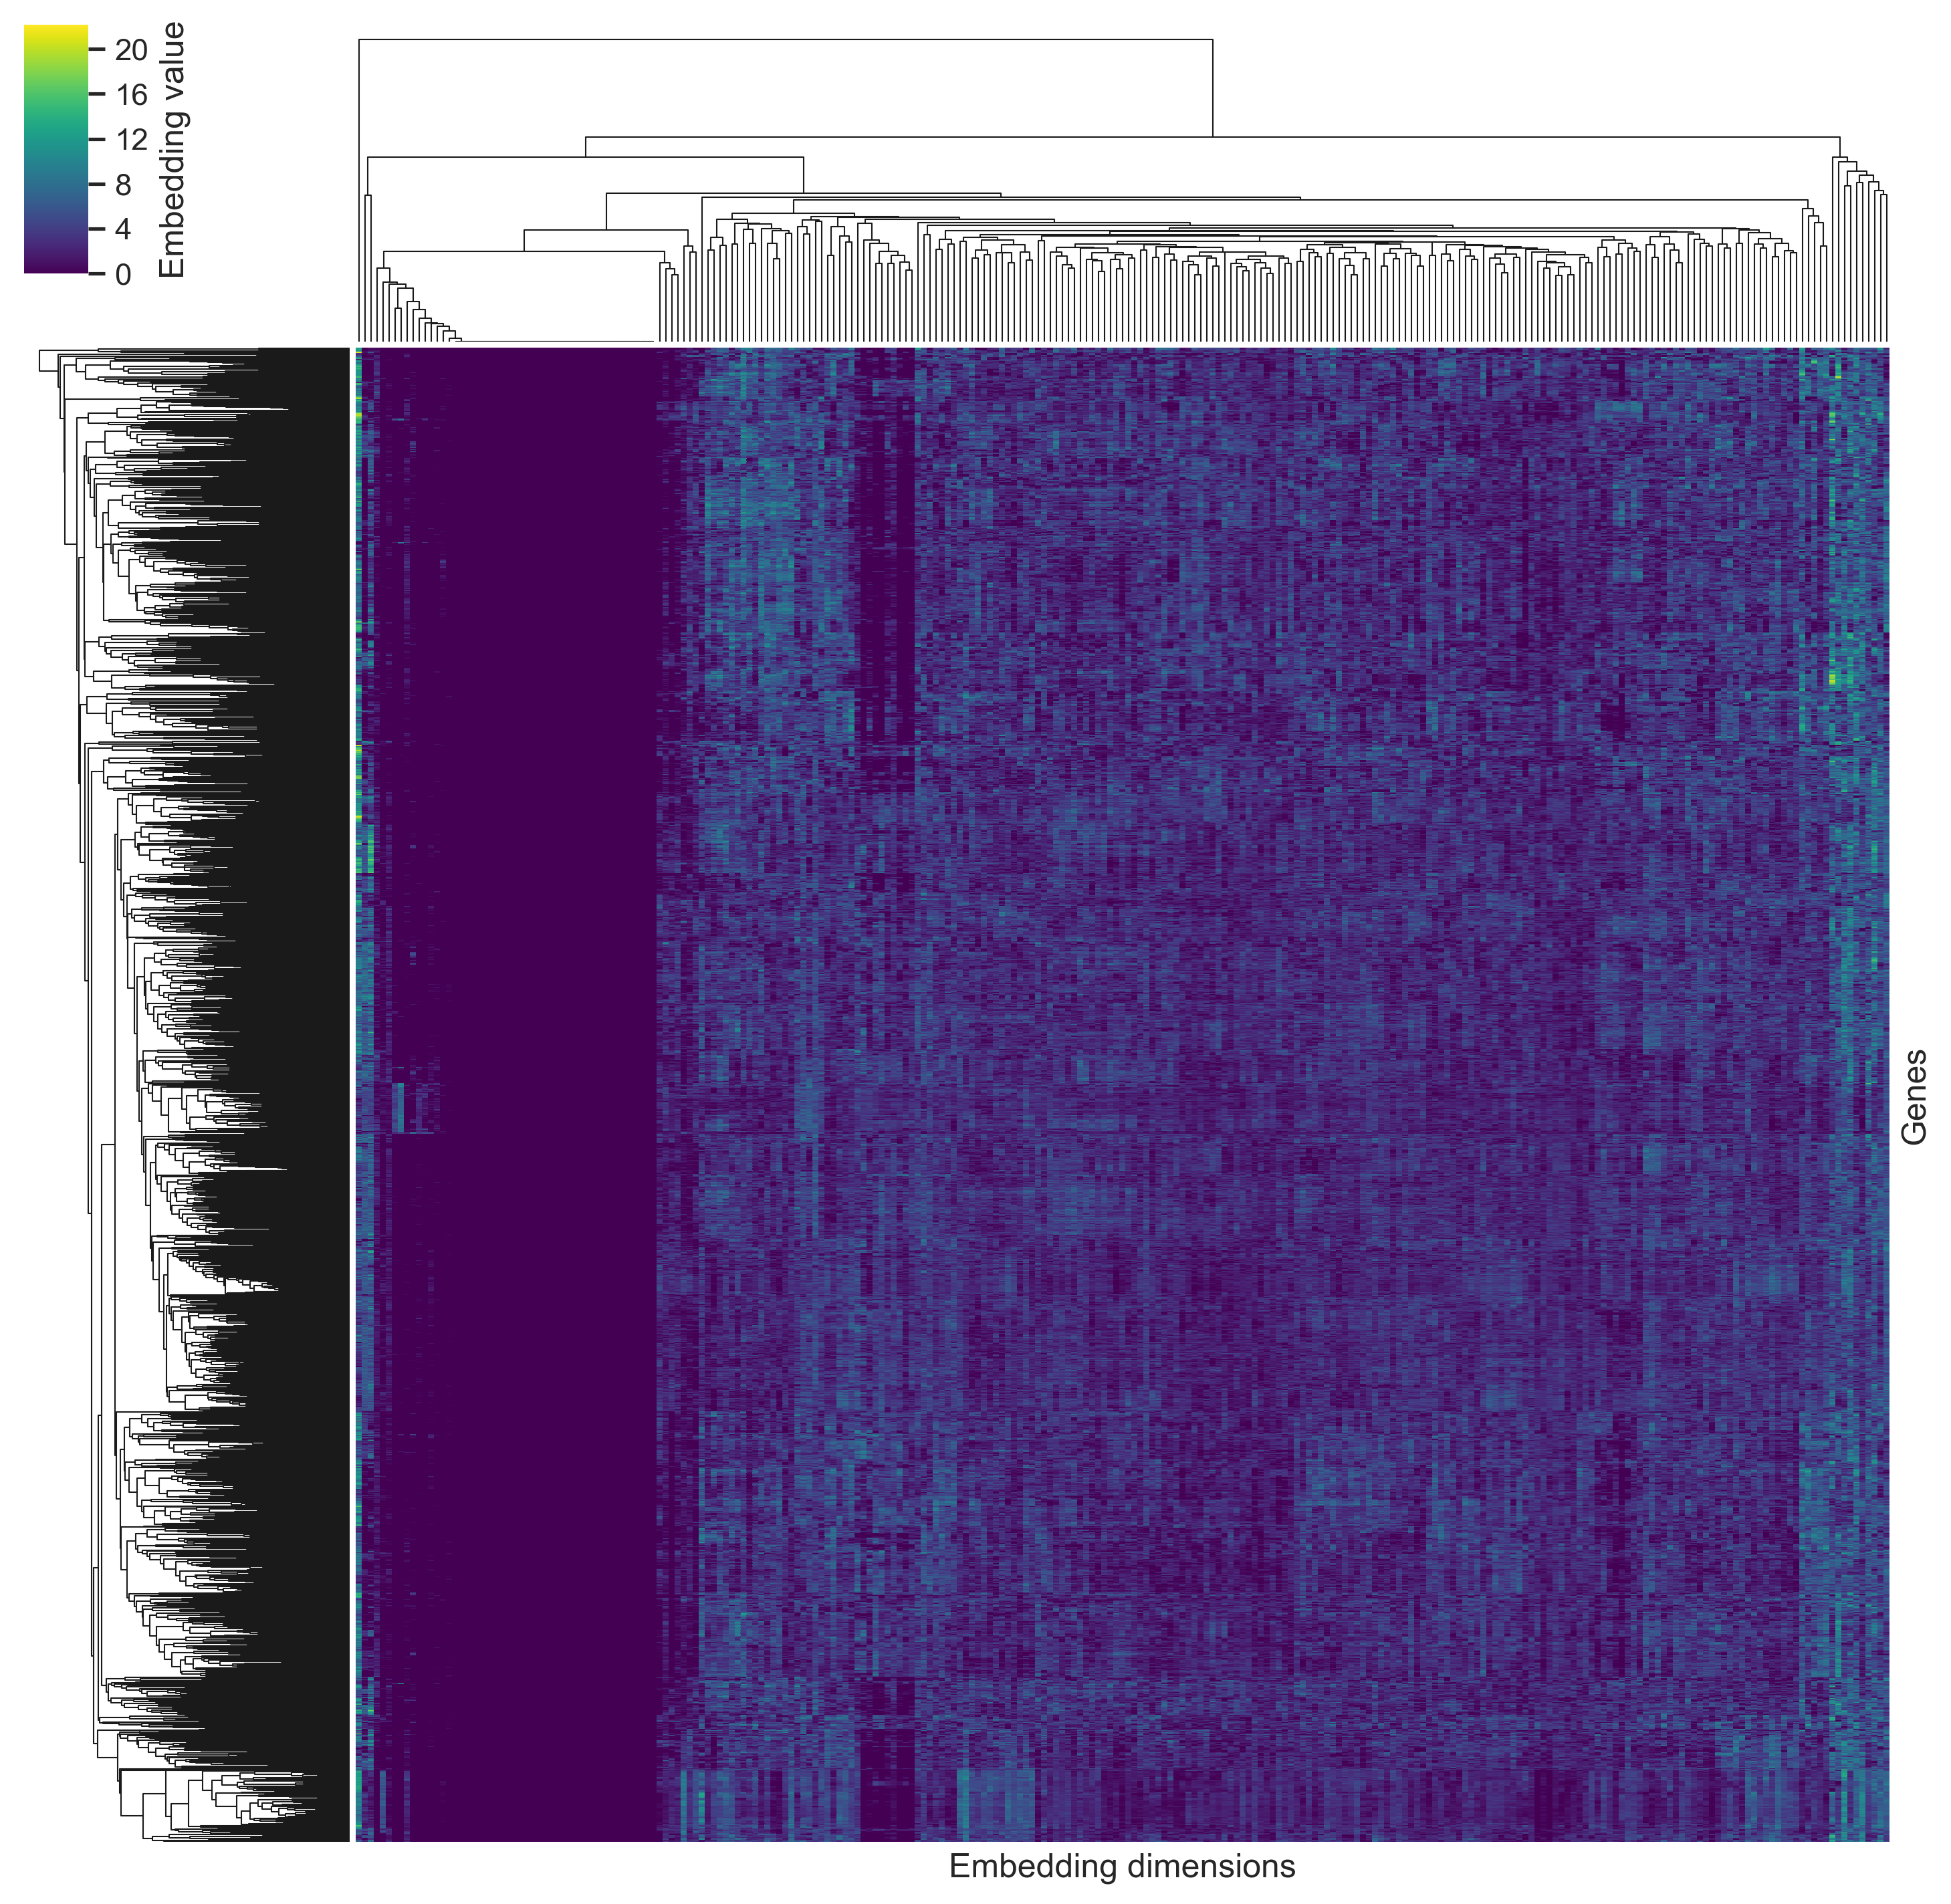
\includegraphics[width=\textwidth]{./Chapter_network_fusion/pombe/autoencoder/network_embeddings}
%     \caption{%
%         Clustered heatmap of \emph{S. pombe} $256$D embeddings.
%         The Euclidean distance matrix was clustered using the
%         % unweighted pair group method using arithmetic averages
%         UPGMA algorithm.
%     }
%     \label{fig:network_embedding_clustermap}
% \end{figure}

\begin{figure}[!hbt]
    \centering
    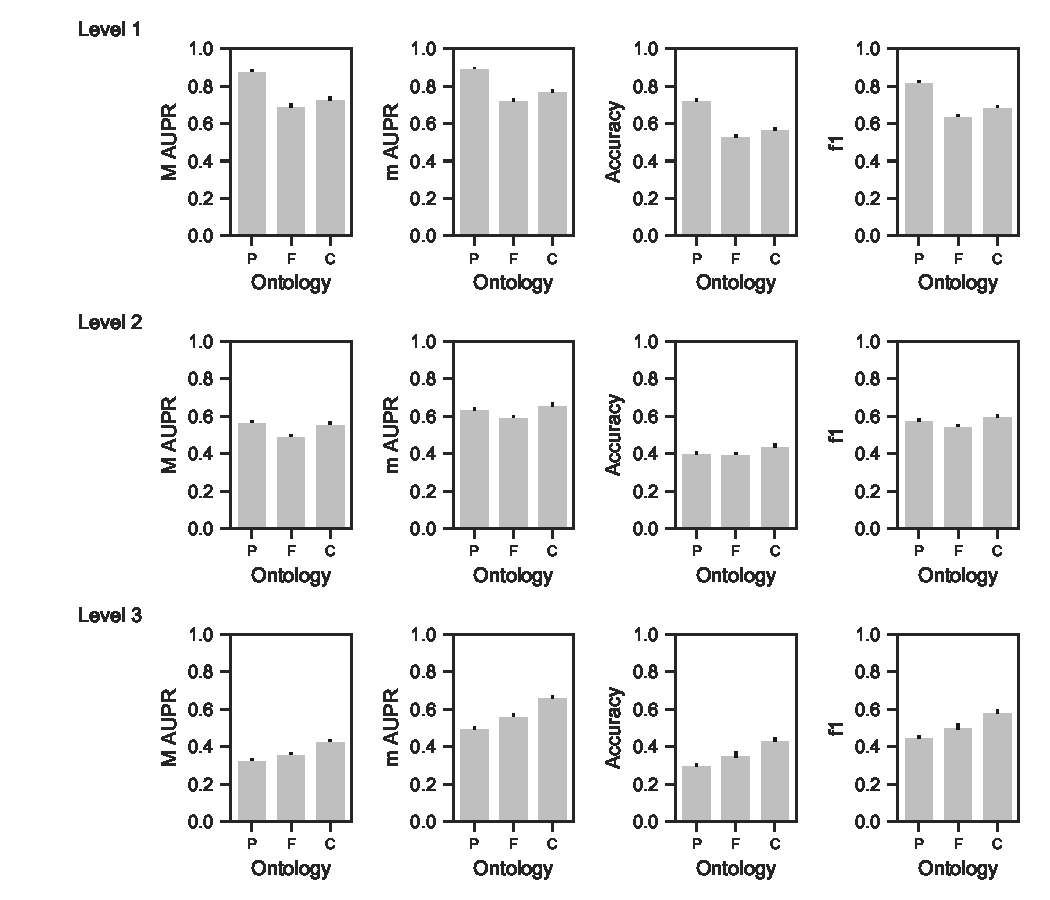
\includegraphics[width=\textwidth]{./Chapter_network_fusion/pombe/mlp/cv_pombe_PFC_9-networks_separate_MLP-512-256}
    \caption{%
        \emph{S. pombe} protein function prediction performance on $256$D embeddings generated by feature learning from nine networks.
        MLPs were trained to predict all GO terms in a level simultaneously.
        GO terms were divided into three levels according to the number of proteins that are annotated with each term.
        Bars are the mean performance across $10$ independent trials of $5$-fold cross-validation and error bars are the standard deviation.
        % Structured prediction of GO annotations for each ontology divided into three levels.
        % All GO terms from an ontology and level level were predicted simultaneously.
        % 256D protein embeddings from a 256-256 MDAE were used as features to train a 512-256 MLP with 0.5 dropout to predict all GO terms in a level simultaneously from the biological process (P), molecular function (F) and cellular component (C) ontologies.
        % GO terms from each ontology were divided into three levels according to the number of proteins that are annotated with each term: 101-300 proteins in level 1, 31-100 proteins in level 2, and 11-30 proteins in level 3. 10 independent trials of 5-fold cross-validation were performed. The mean performance across the independent trials is shown. Error bars show the standard deviation.
    }
    \label{fig:pombe-9-networks-cv}
\end{figure}

% \begin{figure}[!ht]
%     \centering
%     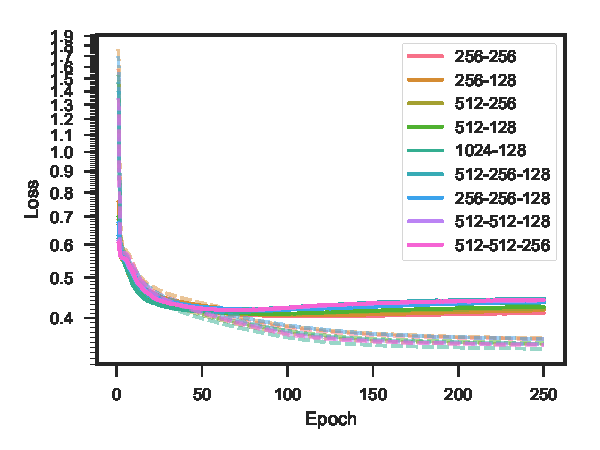
\includegraphics[width=\textwidth]{./Chapter_network_fusion/pombe/autoencoder/architectures_9-networks}
%     \caption{%Reconstruction loss for different MDAE architectures producing 128D and 256D embeddings. \mdaarchitectures MDAs were trained on \emph{S. pombe} data derived from 6 STRING networks, a genetic interaction network, protein expression correlation network and FYPO network. The reconstruction loss was calculated on a validation set consisting of 10\% of the available data.}
%     \label{fig:pombe-9-networks-loss}
% \end{figure}

We also tried fusing three other combinations of data, but could not improve upon the performance of six STRING networks alone.
However, we chose to not show these results because they are similar to \ref{fig:pombe-9-networks-cv} and are highly repetitive
We tested the following combinations:

\begin{enumerate}
    \item six STRING networks, genetic interaction and gene co-expression,
    \item five STRING (not co-expression), genetic interaction and gene co-expression, and
    \item STRING physical interaction network, genetic interaction and gene co-expression.
\end{enumerate}

Combinations 1 and 2 produced slightly lower prediction performance than the six STRING networks.
Combination 3 yielded much worse performance than using six STRING networks.

% \subsubsection{PCNet}\label{pcnet-1}
%
% I used the PCNet integration strategy to combine the \emph{S. pombe} STRING network with the genetic interaction and gene co-expression networks. Note that the FYPO network could not be included, as it is a bipartite network between proteins and terms and does not have any edges in common with the other networks. The \emph{S. pombe} PCNet was used to train a variety of autoencoder (AE, not MDAE) architectures (\ref{fig:PCNet-loss}) and the best architecture was 512-256 AE, with a best validation loss of 0.046.
%
% \begin{figure}[!ht]
%     \centering
%     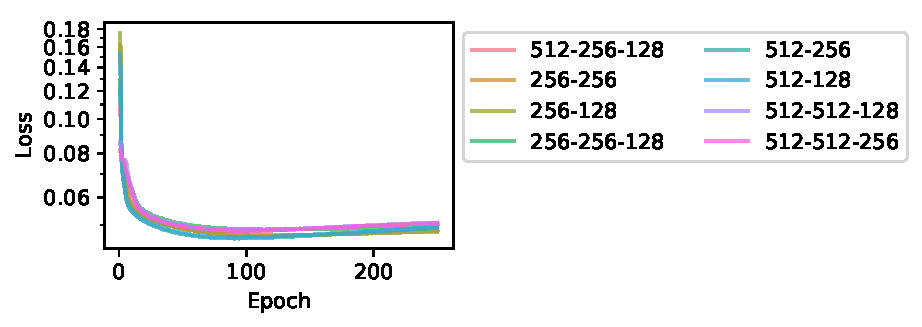
\includegraphics{./Chapter_network_fusion/pombe/autoencoder/architectures_PCNet}
%     \caption{%Losses for different autoencoder architectures producing 128D and 256D embeddings. Autoencoders were trained on a single network derived from the combined \emph{S. pombe} STRING networks, BioGRID physical and genetic interaction networks and a gene expression correlation network with correlations PCC > 0.5 and used to generate gene embeddings. \mdaarchitectures The reconstruction loss was calculated on a validation set consisting of 10\% of the available data.}
%     \label{fig:PCNet-loss}
% \end{figure}
%
% The 256D PCNet gene embeddings were benchmarked (\ref{fig:PCNet-cv}) and found to have a much worse performance than when using an MDAE to fuse the multiple networks. This is an encouraging result that displays the power of MDAs over more traditional methods for data fusion.
%
% \begin{figure}[!ht]
%     \centering
%     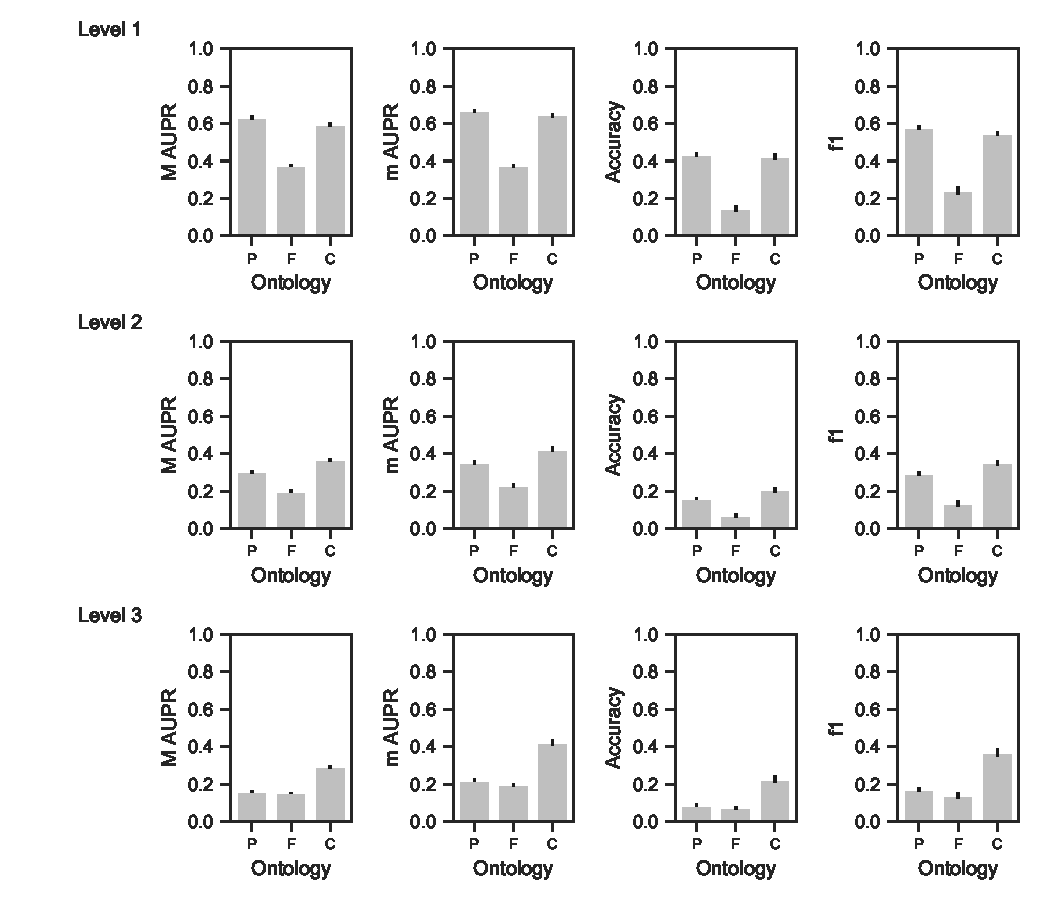
\includegraphics{./Chapter_network_fusion/pombe/mlp/cv_pombe_PFC_PCNet}
%     \caption{%Structured prediction of GO annotations for each ontology divided into three levels. \cvgomlp}
%     \label{fig:PCNet-cv}
% \end{figure}

\section{Discussion}

% MIPS term annotations were predicted for the 6400 proteins in \emph{S. cerevisiae} STRING networks. At the time of performing the work, a newer version of STRING had been released (v 10.5). However, for means of comparison, I used the same version as deepNF (v 9.1). STRING v 9.1 contains 6400 proteins, whereas, v 10.5 has 6391 proteins. This was a source of confusion because the deepNF paper does not specify which version of STRING was used. MIPS is quite an outdated resource whose latest publication is from 2005 \cite{Pagel2005}. deepNF was benchmarked using MIPS annotations so that its performance could be compared to another method, Mashup \cite{Cho2016}, that also predicted MIPS annotations. As such, I also predicted MIPS annotations for \emph{S. cerevisiae}, but I predicted GO annotations for \emph{S. pombe}.

\subsection{Small embeddings achieve comparable performance to deepNF}

deepNF used a $2000$-$600$ MDAE, which contains an unnecessarily large number of parameters to model the amount of information contained in \emph{S. cerevisiae} protein networks.
Models of this size require $\sim 10^6$ examples to train all parameters sufficiently.
Because we only have in the order of $10^3 - 10^4$ proteins as examples, smaller architectures should be used.
We tested whether smaller embeddings of $128$D or $256$D could be used (\ref{sec:experiment-with-different-mda-architectures}).
We found that $256$D were sufficient to replicate the performance of deepNF's $600$D embeddings (\ref{fig:256D-embeddings-SVM-cv}).
Although we were unable to surpass the published performance of deepNF, this is still an improvement over deepNF.
By using smaller embeddings, MDAs, SVMs and MLPs can be trained faster, which is beneficial when performing research using machine learning.

\subsection{Sets of protein functions can be predicted simultaneously using structured learning}

Neural networks can be trained using structured learning, where models output vectors, rather than scalars.
In structured learning, models can predict multiple classes simultaneously, whilst also learning non-linear correlations between sets of features and sets of labels.

We used structured learning to predict \emph{S. cerevisiae} protein function (\ref{structured-prediction-of-mips-annotations}).
We found that structured learning predicts function using $256$D embeddings with comparable performance to deepNF using $600$D embeddings and one-vs-rest SVMs (\ref{fig:levels-cerevisiae-cv}).
On balance, we believe that these moderate reductions in performance are worthwhile, due to the concomitant benefits of structured prediction and the orders of magnitude faster training time compared to one-vs-rest SVMs.

\subsection{Embeddings of yeast proteins predict function}

We applied this model to predict \emph{S. pombe} protein function using $256$D embeddings and structured learning  (\ref{sec:results-pombe}).
We either predicted all terms from an ontology simultaneously, or split terms from each ontology into three levels and predicted separately all terms from each level simultaneously.

For structured learning of levels within an ontology, we predicted cellular component terms consistently well in all three levels.
This is probably due to the wider coverage of experimental annotations for these terms.
Cellular component terms can be experimentally validated easily using simple assays and high-throughput methods.
Conversely, the predictive performance for the biological process ontology is high for level 1, but drops steeply by level 3, which may reflect the comparatively smaller number of proteins with experimental annotations.
These conclusions are recapitulated in an analysis that we conducted into the distribution and quality of \emph{S. pombe} GO annotations in \ref{sec:fission-yeast-known-functions}.
For structured learning of entire ontologies, we obtained a performance approximately the same as the performance for level 3 terms from each ontology, respectively.

Subset accuracy is clearly an inappropriate metric for structured learning tasks.
It is much too strict when predicting a vector of labels.
The other three metrics, however, hold up well under structured learning.

Going forward, one strategy for protein function prediction could be to train an ensemble model, consisting of a structured learning model and a one-vs-rest model.
Classifiers trained using the one-vs-rest strategy would learn patterns that predict individual functions well.
On the other hand, structured learning models would learn non-linear correlations between features and labels to predict subtle, complex functions.
The ensemble model $E$ could combine predictions from the one-vs-rest model $O$ and the structured learning model $S$ using a strategy such as:

\begin{itemize}
    \item Logical OR: $\lor(O = 0, S = 1) = 1$
    \item Max: $\max(O = 0.9, S = 0.4) = 0.9$
    \item Mean: $\text{mean}(O = 0.9, S = 0.4) = 0.65$
\end{itemize}

\subsection{Including orthogonal protein network data did not increase prediction performance}

We tested whether the performance of predicting \emph{S. pombe} protein functions could be improved by including additional, orthogonal protein network data.
We trained MDAs to learn features from different combinations of network data, with and without the six STRING networks used by deepNF.
In all cases, we were unable to improve upon the features learnt from six STRING networks.
Compared to the six STRING networks alone, the reconstruction losses for MDAs trained on different combinations of networks were much higher.
Furthermore, the protein function prediction performance was also much lower when using these different combinations of networks, compared to the six STRING networks alone.

It is unclear why this is the case.
STRING is a trusted resource that is curated to a high-quality.
The six STRING networks may have been processed in some way, such that the six networks correlate well with each other.
Including exogenous data, such as genetic interactions, gene co-expression correlations and experimental phenotypes may not correlate well with the STRING data.
Alternatively, these other three types of interaction data may be more noisy than STRING data, due to the nature of the data, how it was processed, or the level to which the database has been curated.

In the future, it will be interesting to see whether additional, orthogonal types of interaction data can be fused together successfully.
Protein functional association resources continue to improve as measurement accuracies increase, large-scale experiments become commonplace and previous experimental results are independently validated.

\subsection{Conclusion}

The work in this chapter successfully replicated the published performance of a novel protein function prediction method, deepNF, that uses MDAs and protein network data to generate embeddings of proteins.
We then improved upon deepNF in three ways.
Firstly, we showed that smaller MDAE architectures, and secondly, smaller embedding dimensions, achieve comparable performance to deepNF.
Thirdly, we found that protein functions can be predicted using structured learning with the same performance as predicting each function using a separate classifier.
This reduced training and prediction time, whilst also allowing non-linear correlations to be learnt between features and labels.
We applied our improved model to successfully predict \emph{S. pombe} protein function using structured learning.
We use this approach in \ref{chapter:yeast}, in combination with phenotypic and protein evolution data, to predict \emph{S. pombe} protein function.

% \references
